\chapter{Dynamical Systems}
\label{ch-dynamical-sys}

This chapter is mainly based on 
Refs.\cite{dynamical-fuchs} and \cite{wiki-phase-plane}.

{\bf Dynamical Systems} (DS)
is the study of systems of one or more
coupled 1st order (i.e., no derivatives higher than 1st order allowed) {\bf Ordinary Differential Equations} (ODE).
The constraint of allowing only 1st order
derivatives does not result in any loss of generality,
because, as we shall see below, higher order ODE
can always be replaced by multiple 1st order ODEs.
Hence, DS studies a vector equation
\beq
\underbrace{\frac{d\vec{x}}{dt}}_{\dot{\vec{x}}}
= \vec{f}(\vec{x}, t)
\eeq
where $\vec{x},  \vec{f}\in\RR^n$ for nD (i.e., n-dimensions)
If $\vec{f}(\vec{x},t)$
depends explicitly on $t$ 
the ODE is said
to describe an {\bf autonomous
system}.
If it does depend on $t$,
it is said to describe a
{\bf non-autonomous or driven
system}.

A {\bf fixed point} is defined as a point
at which $\dot{\vec{x}}=0$.

One can draw a bnet for a DS wherein some
of the nodes are the components of $\vec{x}$
and other nodes are the components of $\dot{\vec{x}}$.
The bnets of DS allow one to describe feedback and time
varying processes in the continuous time limit.
Other ways of describing time varying processes, albeit in the
discrete time regime, are Dynamical Bnets (see Chapter \ref{ch-dyn-bnets}),
Time Series Analysis (see Chapter \ref{ch-time-arma})
and Petri Nets (see Chapter \ref{ch-petri}).


Often a DS can be in a parameter region
in which it is highly sensitive to initial conditions. In such cases, random external noise 
might become important. Those cases are 
addressed by Stochastic Differential Equations (see Chapter
\ref{ch-stochastic-diff-eqns})
ad Chaos Theory.

Control Theory (see Chapter \ref{ch-control-th}) (CT)
and DS deal with the same subjects, but CT is more
engineering oriented whereas DS is more math oriented.
\section{Potential Function}

In 1D, define the {\bf potential function} $V$ by
\beq
f(x,t) = -
\underbrace{\pder{V}{{x}}}_{ \partial_xV}
\eeq
Hence,

\beq
V - V_0= -\int^x_{x_0} dx \; f(x, t)
\eeq

Note that this is not the potential of Newtonian mechanics.\footnote{Let $V_N$ and $F_N=\ddot{x}=-\partial_x V_N$ be the potential and force in
Newtonian mechanics. Furthermore,
assume the simple case $f=\lam x$. Then $\boxed{V=-\lam x^2/2}$. Also
$F_N=m \ddot{x} =m\dot{f}=
m(\partial_x f )\dot{x}=
m\lam^2 x$. Hence $\boxed{V_N = -m\lam^2 x^2/2}$.
So $V_N$,
contrary to $V$, is insensitive to the sign of $\lam$. If $m$, $x$, $t$ have
dimensions of mass, length and time, then
$[f]=\frac{[x]}{[t]}$ and $[V]=[f][x]=\frac{[x]^2}{[t]}$.
On the other hand, $[V_N]=[m\ddot{x}][x]=
\frac{[x]^2[m]}{[t]^2}$.
}



Note that
\beq
\partial_x V = 0 \iff \dot{x}=0
\eeq
and
\beq
\partial^2_x V = -\frac{d\dot{x}}{dx}
\eeq
As shown in Fig.\ref{fig-V-derivatives},
$V$ has positive second derivative
(hold water convexity)
on both sides of a {\bf stable, attractive fixed  point (attractor, sink)},
and it has negative second derivative
(drop water convexity)
on both sides of an {\bf unstable, repulsive fixed point (repeller, source)}. Hence, we can think of
$V$ as a potential in which a ball rolls towards an attractor
and away from a repeller.

Besides being an attractor or a repeller, a fixed point can be a
{\bf saddlepoint}. A saddlepoint
attracts in some directions and repel in others. 

A {\bf monostable/bistable/multistable}
system has one/two/multiple
attractors.

In this book, attractors will be symbolized by a black filled circle (like a black hole). Repellers will 
symbolized by a white (or yellow)  filled circle (like a sun).
Saddle points will be
symbolized by a circle that
is filled half in black
and half in white.


\begin{figure}[h!]
\centering
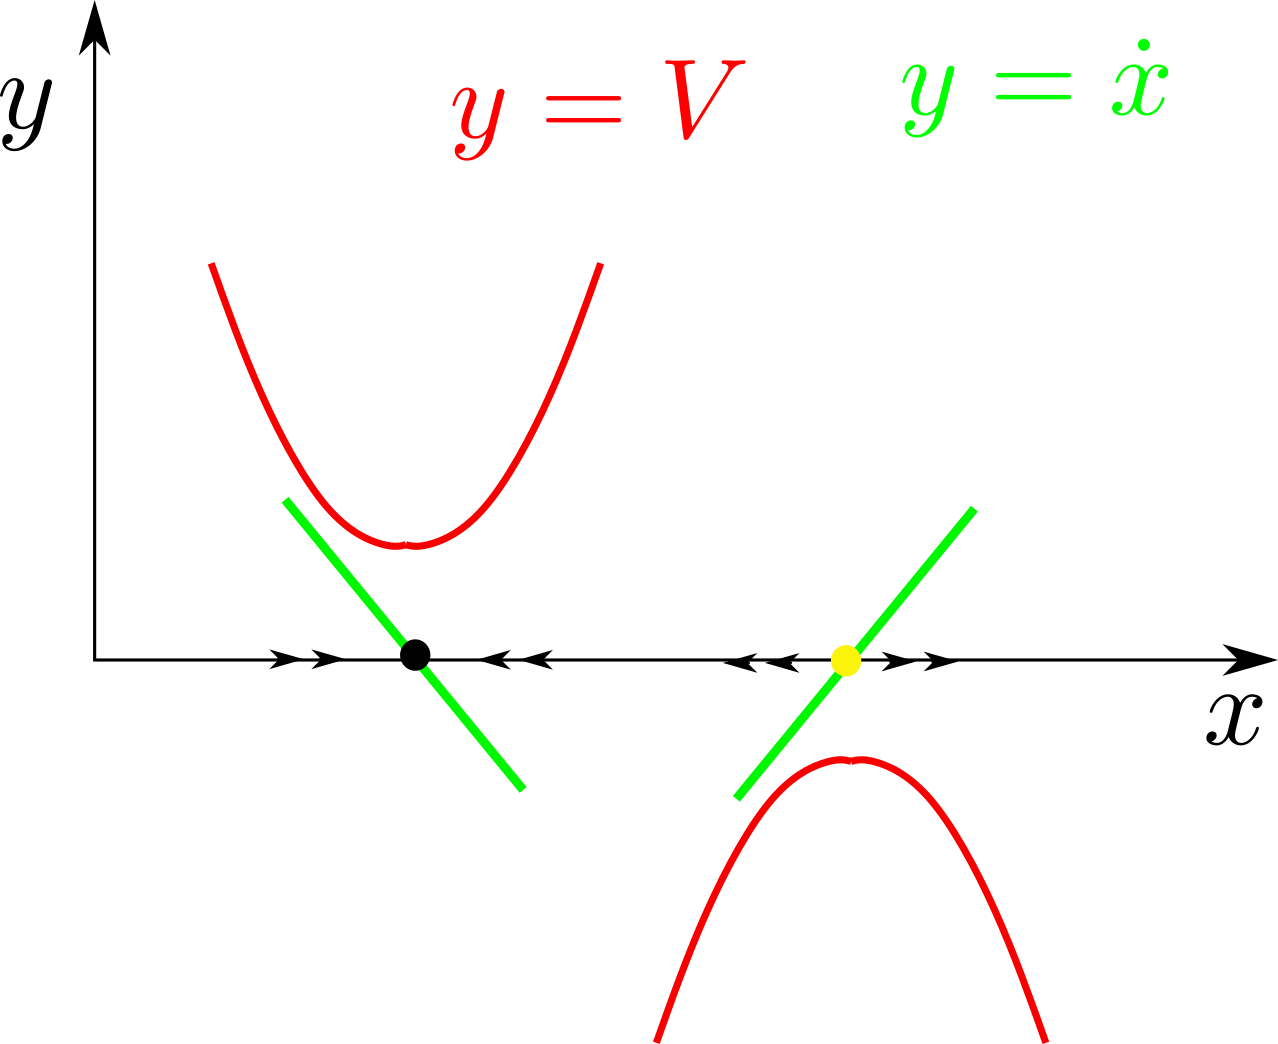
\includegraphics[width=4in]
{dynamical-sys/V-derivatives.png}
\caption{Illustration of
$\frac{d\dot{x}}{dx}=-\partial^2_xV$}
\label{fig-V-derivatives}
\end{figure}

In more than 1D, 

\beq
\dot{\vec{x}} = \vec{f}(\vec{x}, t)
\eeq

\beq
\vec{f}(\vec{x}, t) = -\nabla V
\eeq

\beq
\nabla V=0 \iff \dot{\vec{x}}=0
\eeq

\beq
\nabla^2 V = -\nabla \cdot \dot{\vec{x}}
\eeq

But note that not all $\vec{f}$
can be expressed as a gradient.
In 2D, suppose $\vec{f}=(f_x, f_y)^T$.
If

\beq
\left\{
\begin{array}{{l}}
f_x = \partial_x V
\\
f_y = \partial_y V
\end{array}
\right.
\eeq
then  we must have

\beq
\partial_y f_x =\partial_x f_y
\eeq
because $\partial_x\partial_y V=
\partial_y\partial_x V$.

In 3D, for 

\beq
\vec{f}=\nabla V
\eeq
to be true, we must have

\beq
\nabla\times \vec{f}
=0
\eeq
because $\nabla\times \nabla V=0$ (i.e., a gradient field has no curl)

\section{Phase Portraits}


An N dimensional system described by 
coordinates $q_i$ for $i=1,2, \ldots, N$ 
is said to occupy a point $(q_1, q_2, \ldots, q_N)\in\RR^{N}$
in  {\bf configuration space}
and a point \\$(q_1,\dot{q_1}, q_2, \dot{q_2}\ldots, q_N, \dot{q_N})\in \RR^{2N}$
in {\bf phase space}.  The coordinates of phase 
space are often called {\bf state variables}.

The terms 
{\bf phase portrait} (PP) and 
{\bf phase plane plot} (PPP) are often used interchangeably
although PPP is restricted by its name to be a 2D plot,
whereas the name PP also allows for the possibility  of 3D plots.
We will use the term PP henceforth.

A PP in 2D refers to one of 2 things
\begin{enumerate}
\item a 2D plot of
multiple solutions $(x(t), y(t))$
 (a.k.a. {\bf streamlines}, {\bf trajectories})
for a dynamical system,
where $x,y$ are any two state 
variables of the system.\footnote{
Streamline plots can be drawn using the Python function {\tt matplotlib.pyplot.streamplot}}

\item a 2D plot of a {\bf velocity vector field}, wherein a scaled 
velocity vector  
$(\dot{x}, \dot{y})$ is plotted at each point $(x,y)$
on a 2D mesh.\footnote{Vector field plots can be drawn using the Python function {\tt
matplotlib.pyplot.quiver}}
\end{enumerate}
Items 1 and 2 convey the same
type of intuition about dynamical systems.
In this chapter we use 1, 
but most of what we say about 1 also applies to 2.

A very useful addendum to a PP is to draw in it the lines 
which have either $\dot{x}=0$ or $\dot{y}=0$. These 2 lines are
called the
{\bf nullclines} of the PP.
The points at which the two nullclines intersect
are called {\bf fixed points}.\footnote{Note that it's impossible to travel along a nullcline because, for example, the $\dot{x}$ nullcline contains points 
with different $x$ and it's
impossible to change $x$ in time while $\dot{x}=0$.}


PPs can of course be generalized to 3 or more dimensions.
In the 3D case, 
a PP becomes either
a bunch of 3D streamlines or a 3D velocity vector  field.

Note that if a dynamical system is described by the 
system of ODE:

\beq 
\left\{
\begin{array}{c}
\dot{x}= f(x,y)
\\
\dot{y} = g(x, y)
\end{array}
\right.
\eeq
then one can use the
same software
that we use to draw a PP for $(x,y)$ 
 to draw a PP for
$(x, \dot{x})$.
$x, \dot{x}, y, \dot{y}$
are all considered state variables,
and any pair of them is amenable to a PP.
To draw a PP for $(x, \dot{x})$,
define

\beq
\left\{
\begin{array}{l}
\dot{x} = v
\\
\dot{v} = \pder{f}{x}
\underbrace{\dot{x}}_{f(x,y)} + \pder{f}{y}
\underbrace{\dot{y}}_{g(x,y)}
\\
\dot{y} = g(x, y)
\end{array}
\right.
\label{eq-3d-sys}
\eeq

Note that to arrive at Eq.(\ref{eq-3d-sys})
we  used the same trick that is used to 
express a second order differential equation
of the form

\beq
\ddot{x} = F(x, \dot{x})
\label{eq-2nd-order-ode}
\eeq
as a system of 2 first order ODE.
In that case, we express Eq.(\ref{eq-2nd-order-ode})
as

\beq
\left\{
\begin{array}{l}
\dot{x}=v
\\
\dot{v} = F(x, v)
\end{array}
\right.
\eeq

\OtoAd




\section{Fixed Points in 1D Systems}
\subsection{Linear System}

Consider the system

\beq
\xymatrix{
&\rvx\ar[d]
\\
&\dot{\rvx}
}
\quad
\left\{\dot{x} = \lam x
\right.
\eeq
where $\lam\in\RR$.

For this system,
\beq
V = -\;\frac{\lam}{2}x^2
\eeq 

Fig.\ref{fig-phase-V-linear}
shows $(x, \dot{x})$ and $(x, V)$ plots for the linear
system $\dot{x}=\lam x$.

\begin{figure}[h!]
\centering
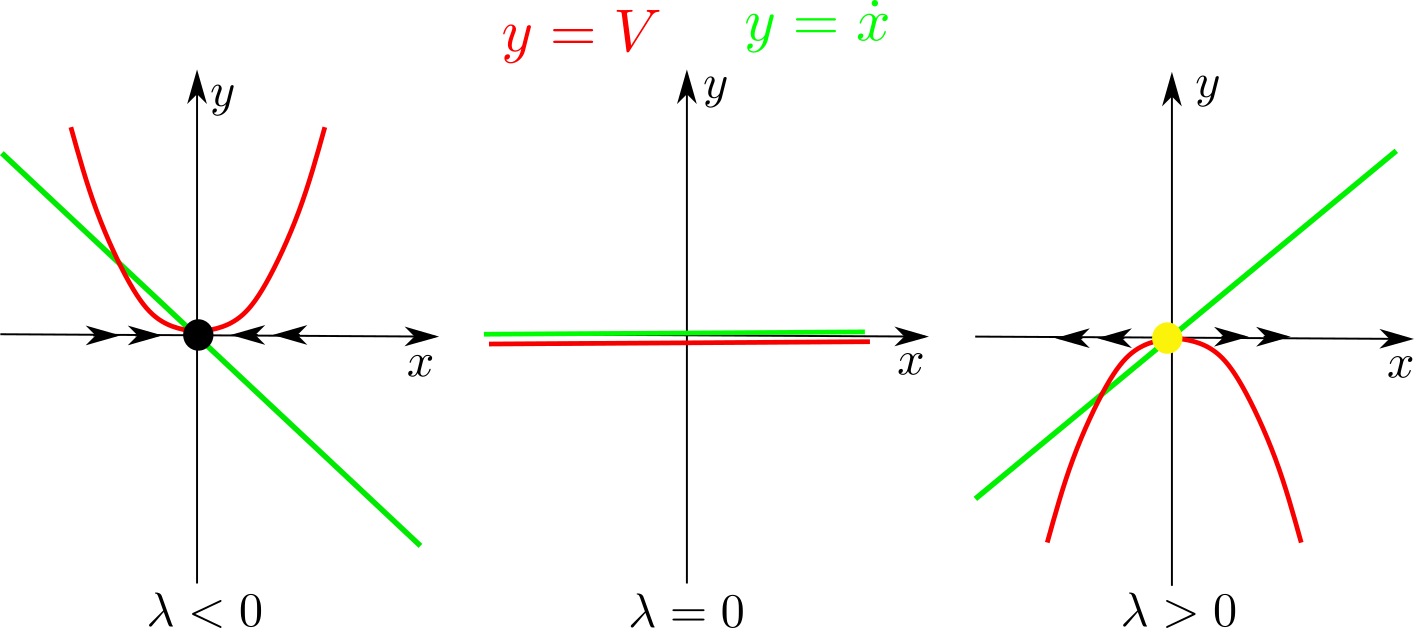
\includegraphics[width=4in]
{dynamical-sys/phase-V-linear.png}
\caption{$(x, \dot{x})$ and $(x, V)$ plots for the linear
system $\dot{x}=\lam x$.}
\label{fig-phase-V-linear}
\end{figure}


\subsection{Quadratic System}

Consider the system 
\beq 
\xymatrix@R=.5pc{
&\rvx\ar[dd]
\ar[dl]
\\
\rvx^2\ar[dr]|\redminus
\\
&\dot{\rvx}
}
\quad
\left\{
\dot{x} = \lam x - x^2
\right.
\eeq
where $\lam\in\RR$.

For this system

\beq
V =-\; \frac{\lam}{2}x^2  + \frac{1}{3} x^3
\eeq 

Fig.\ref{fig-phase-V-quadratic} shows $(x, \dot{x})$ and $(x, V)$ plots for the quadratic
system $\dot{x}=\lam x-x^2$.

\begin{figure}[h!]
\centering
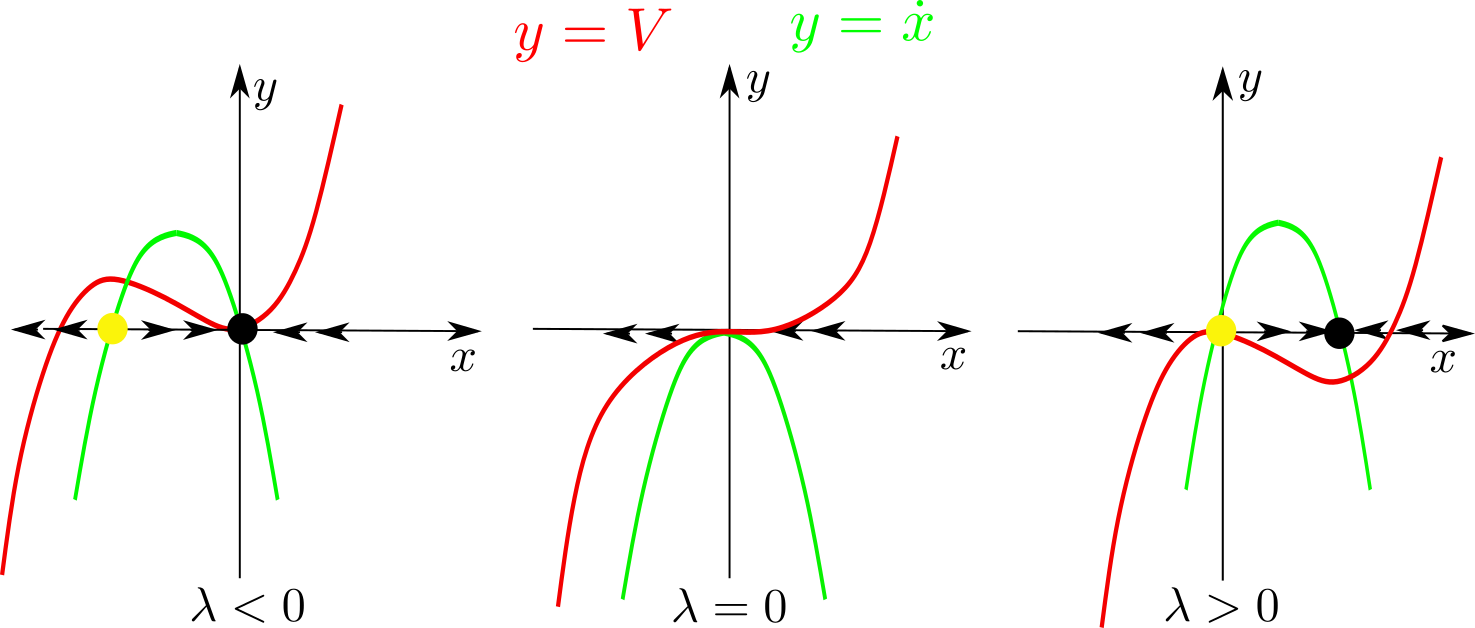
\includegraphics[width=4in]
{dynamical-sys/phase-V-quadratic.png}
\caption{$(x, \dot{x})$ and $(x, V)$ plots for the quadratic
system $\dot{x}=\lam x-x^2$.}
\label{fig-phase-V-quadratic}
\end{figure}

\subsection{Cubic System}

Consider the system
\beq
\xymatrix@R=.5pc{
&\rvx\ar[dd]
\ar[dl]
\\
\rvx^3\ar[dr]|\redminus
\\
&\dot{\rvx}&\ar[l]
}
\left\{
\dot{x} = v_0 + \lam x - x^3
\right.
\eeq
where $\lam, v_0\in\RR$. 

For this system

\beq
V = -v_{0}x -\;\frac{\lam}{2}x^2  + \frac{1}{4} x^4
\eeq

Assume $\lam =1$, $\dot{x}=0$. Then

\beq
x^3=v_0 + x
\label{eq-fp-cubic}
\eeq
Fig.\ref{fig-geometrical-v-critical-v0} shows a plot of the line and cubic

\beq 
\left\{
\begin{array}{l}
y=v_0 + x
\\
y= x^3
\end{array}
\right.
\eeq
Eq.(\ref{eq-fp-cubic})
is satisfied precisely
when this line and
cubic  intersect.
For large $|x|$,
these 2 curves intersect
at a single point. For $x=0$,
they intersect at 3 points.
In between,
 when the line kisses the 
 cubic at one point, 
 there are 2 intersections and
 therefore 2 solutions to 
 Eq.(\ref{eq-fp-cubic}).
Call $(x_c, y_c)$
and $(-x_c, -y_c)$
with $x_c, y_c\geq 0$,
the two 
points at which
the cubic and the 
line kiss.
A closed expression
for $x_c$ and $y_c$ can
be found,
but it's complicated (it
involves the solution of a cubic
equation). Suffice it to say that we have proven the
existence of
$x_c, y_c$ and their values can be easily found numerically by computer.
When $(x, \dot{x}) = (\pm x_c, \pm y_c)$, we say that the
system is at a {\bf critical point}
and we call $v_c=y_c$
the {\bf critical velocity}.

Fig.\ref{fig-phase-V-cubic-zero-v0} shows plots of $(x, \dot{x})$ and $(x, V)$ for the cubic system
$\dot{x}=v_0 + \lam x-x^3$ with $v_0=0$
whereas Fig.\ref{fig-phase-V-cubic-with-v0} shows them when 
$v_0\neq 0$ and $\lam=1$.
When $v_0=0$ there is no critical point, whereas when $v_0\neq 0$ there is.

Fig.\ref{fig-rolling ball}
presents an interpretation
of the critical velocity 
$v_c$ in terms
of the potential $V$.

\begin{figure}[h!]
\centering
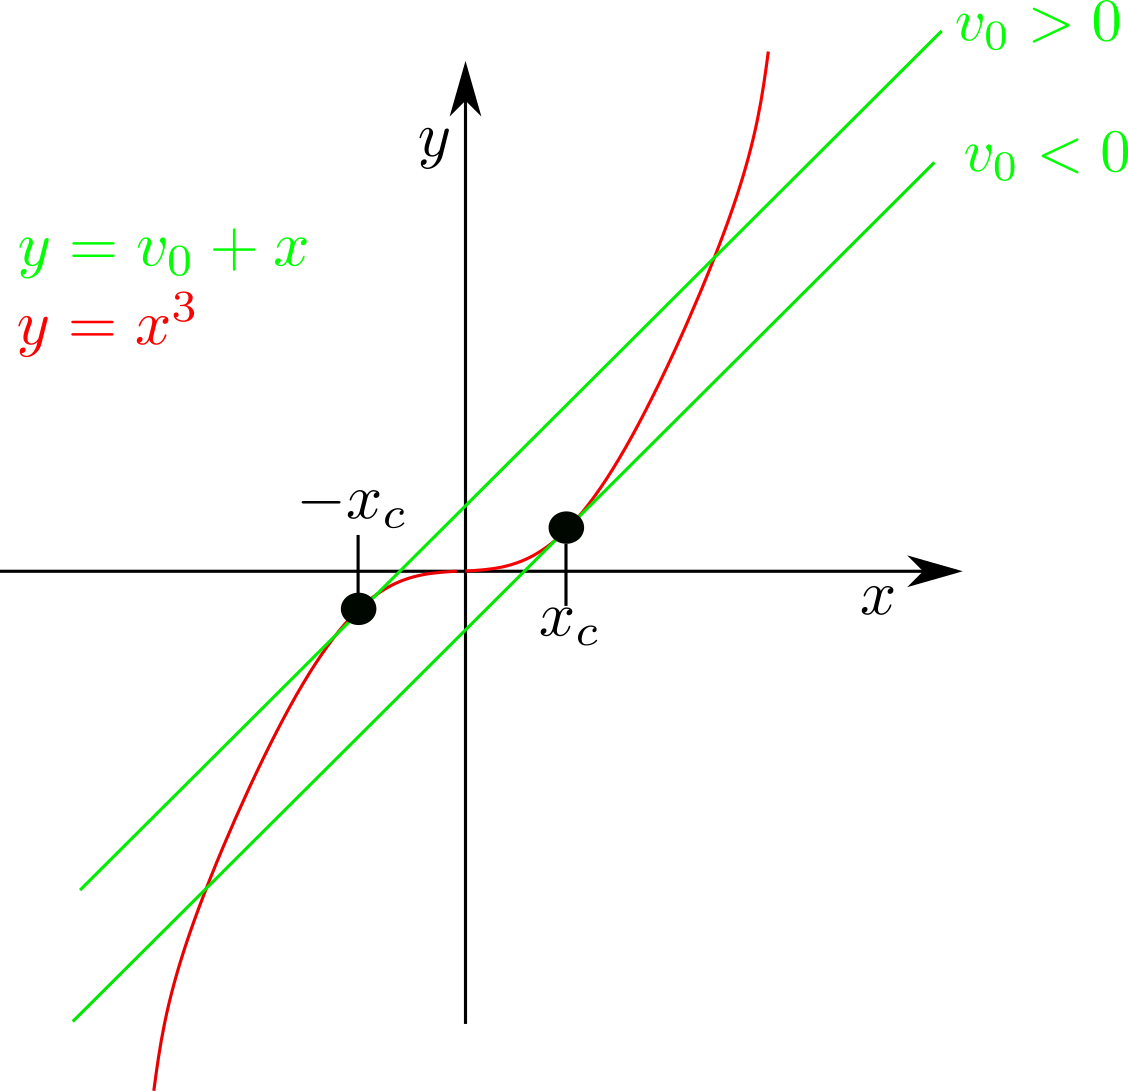
\includegraphics[width=2.5in]
{dynamical-sys/geometrical-v-critical.png}
\caption{$(\pm x_c, \pm y_c)$
are the two points at which 
the line
$y=v_0 + x$ and the cubic
$y=x^3$
kiss.
}
\label{fig-geometrical-v-critical-v0}
\end{figure}


\begin{figure}[h!]
\centering
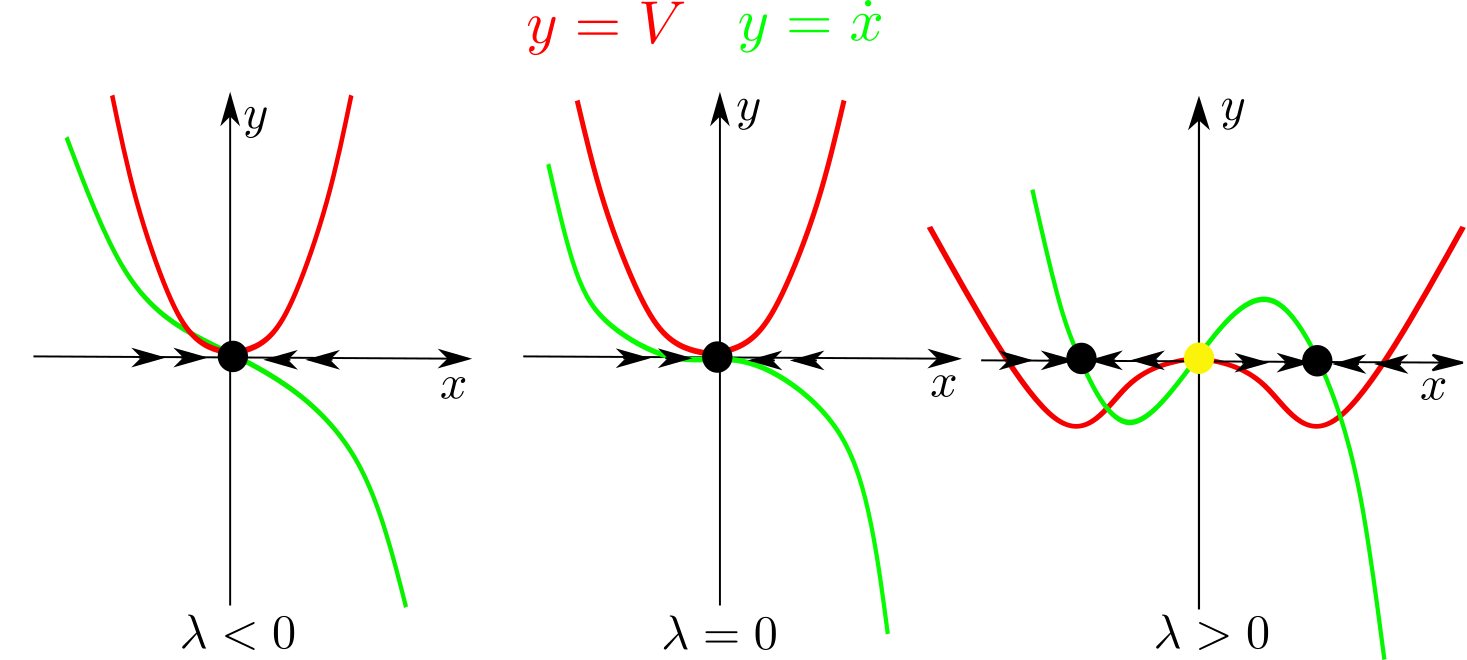
\includegraphics[width=4in]
{dynamical-sys/phase-V-cubic-zero-v0.png}
\caption{$(x, \dot{x})$ and $(x, V)$ plots for the cubic system
$\dot{x}=v_0 + \lam x-x^3$ with $v_0=0$.}
\label{fig-phase-V-cubic-zero-v0}
\end{figure}

\begin{figure}[h!]
\centering
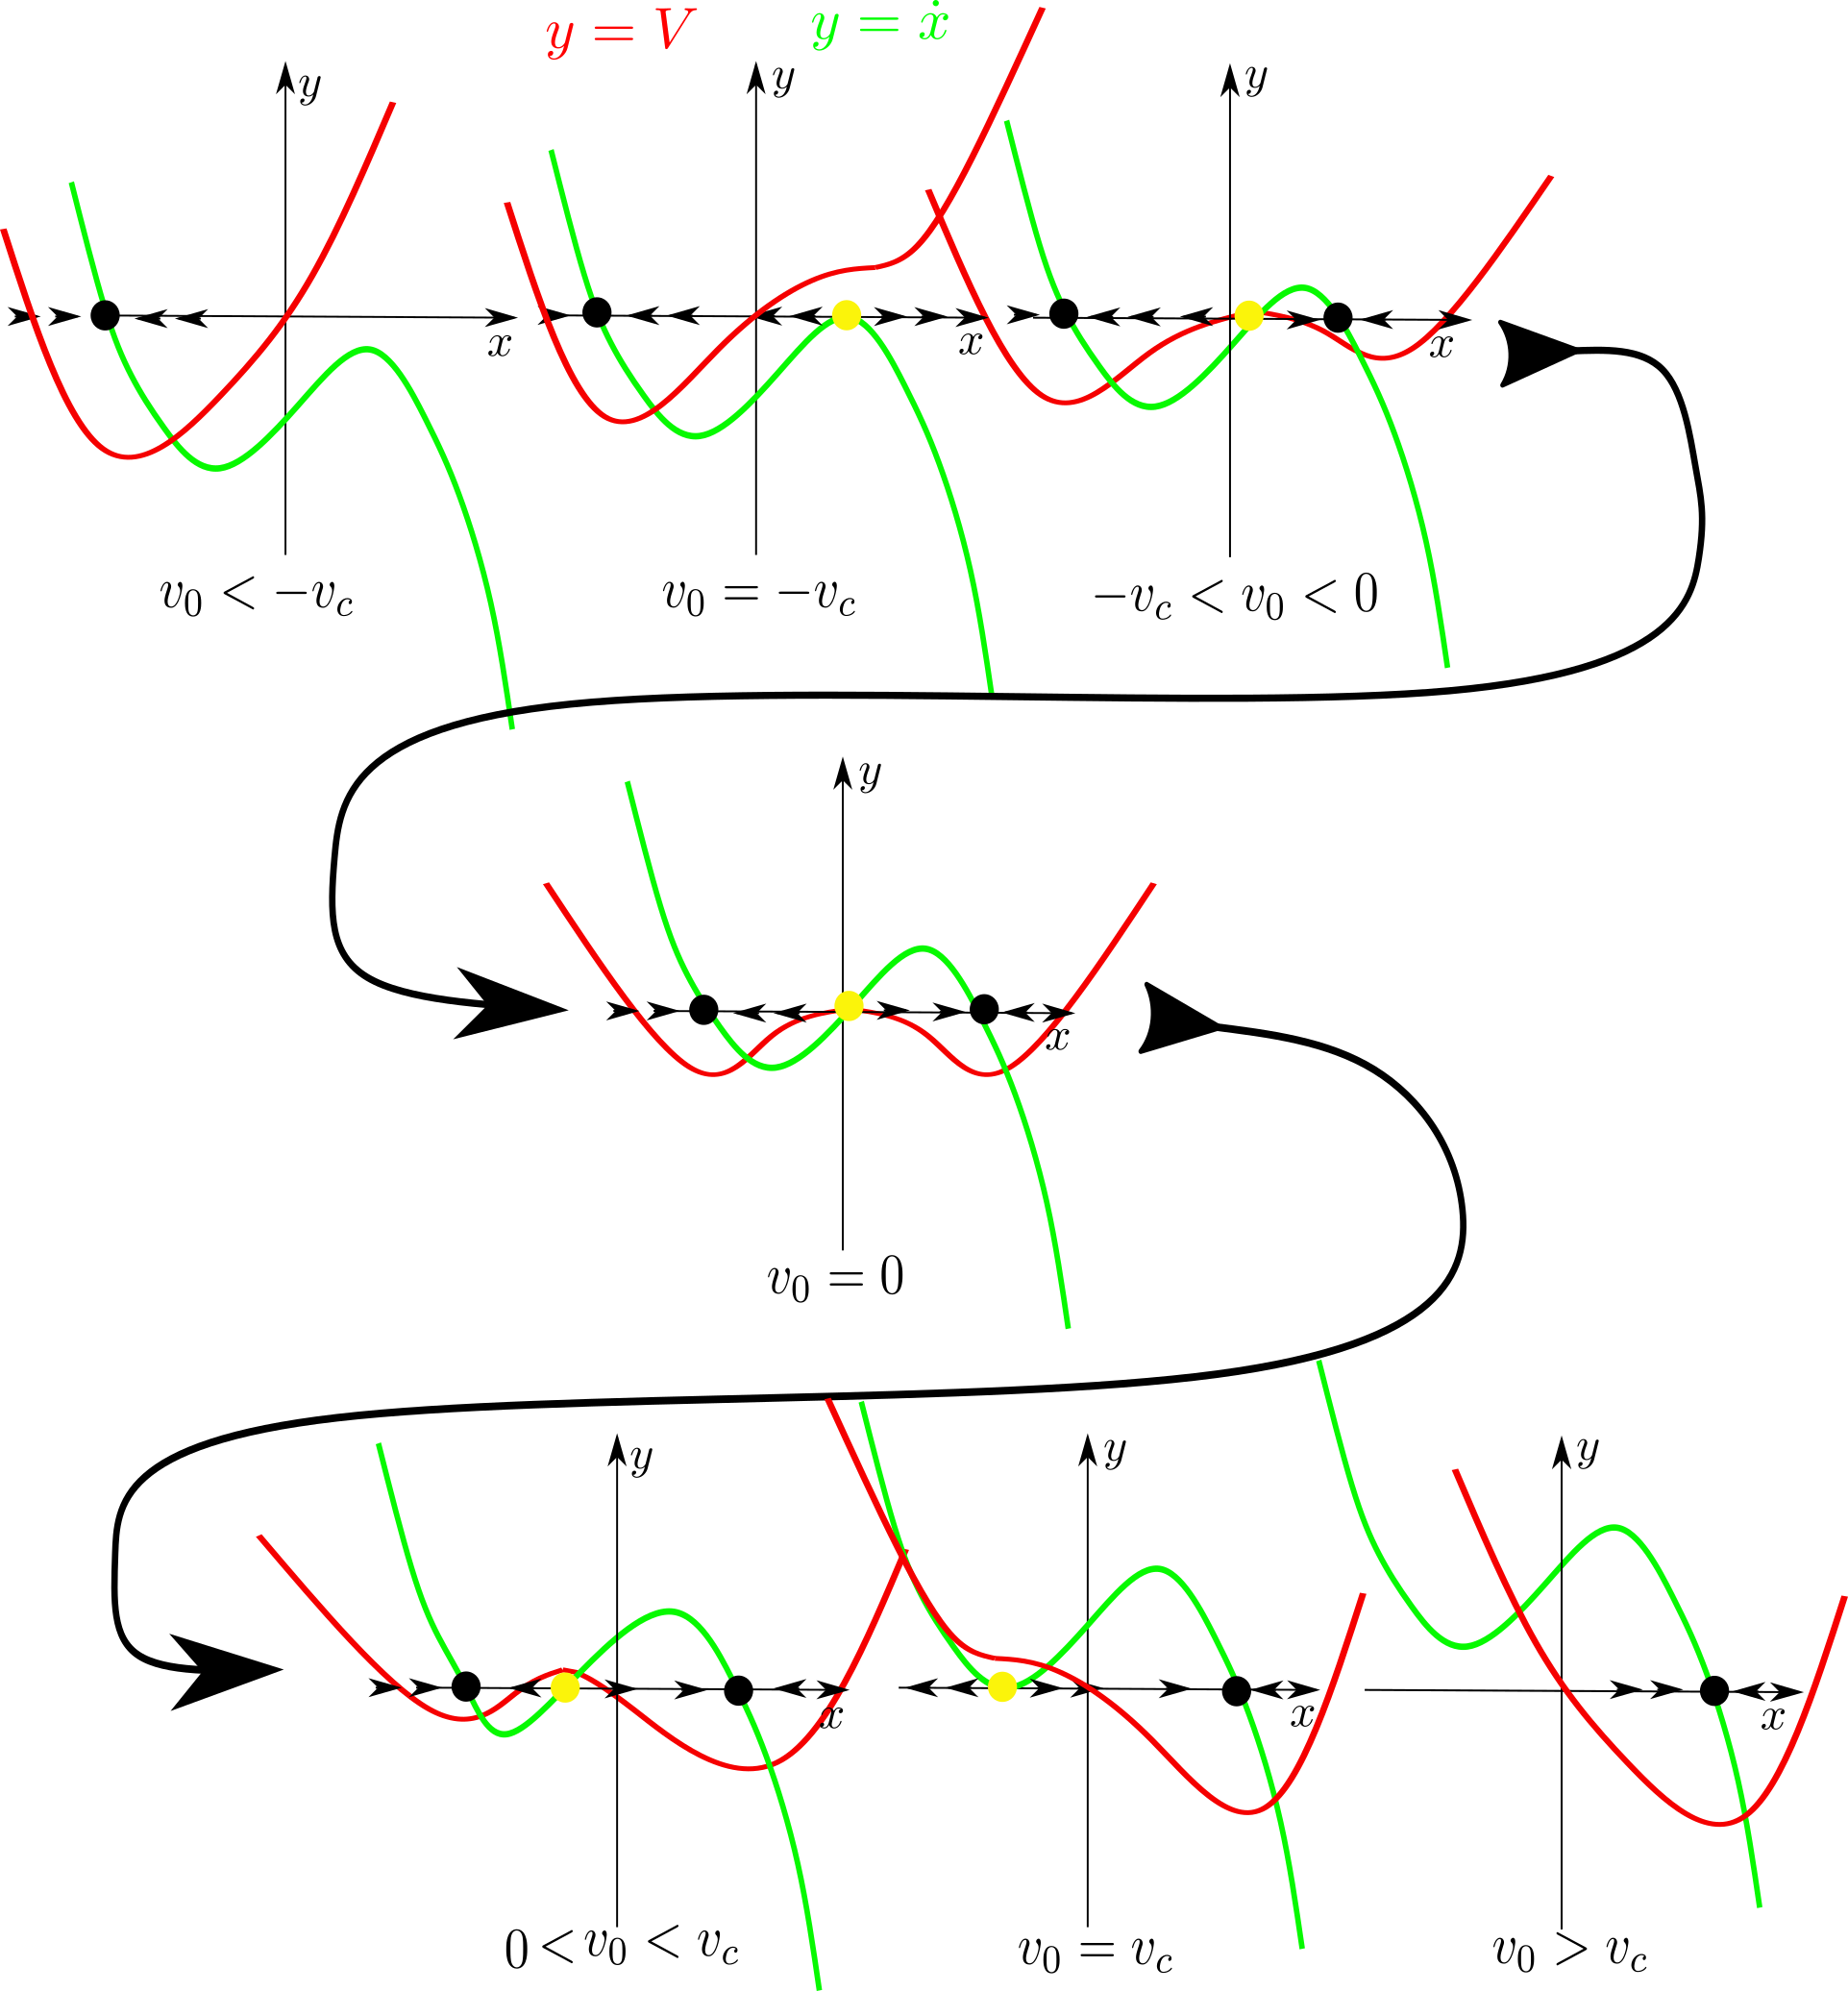
\includegraphics[width=4in]
{dynamical-sys/phase-V-cubic-with-v0.png}
\caption{$(x, \dot{x})$ and $(x, V)$ plots for the cubic system
$\dot{x}=v_0 + \lam x-x^3$ with $v_0\neq 0$
and $\lam=1$.}
\label{fig-phase-V-cubic-with-v0}
\end{figure}

\begin{figure}[h!]
\centering
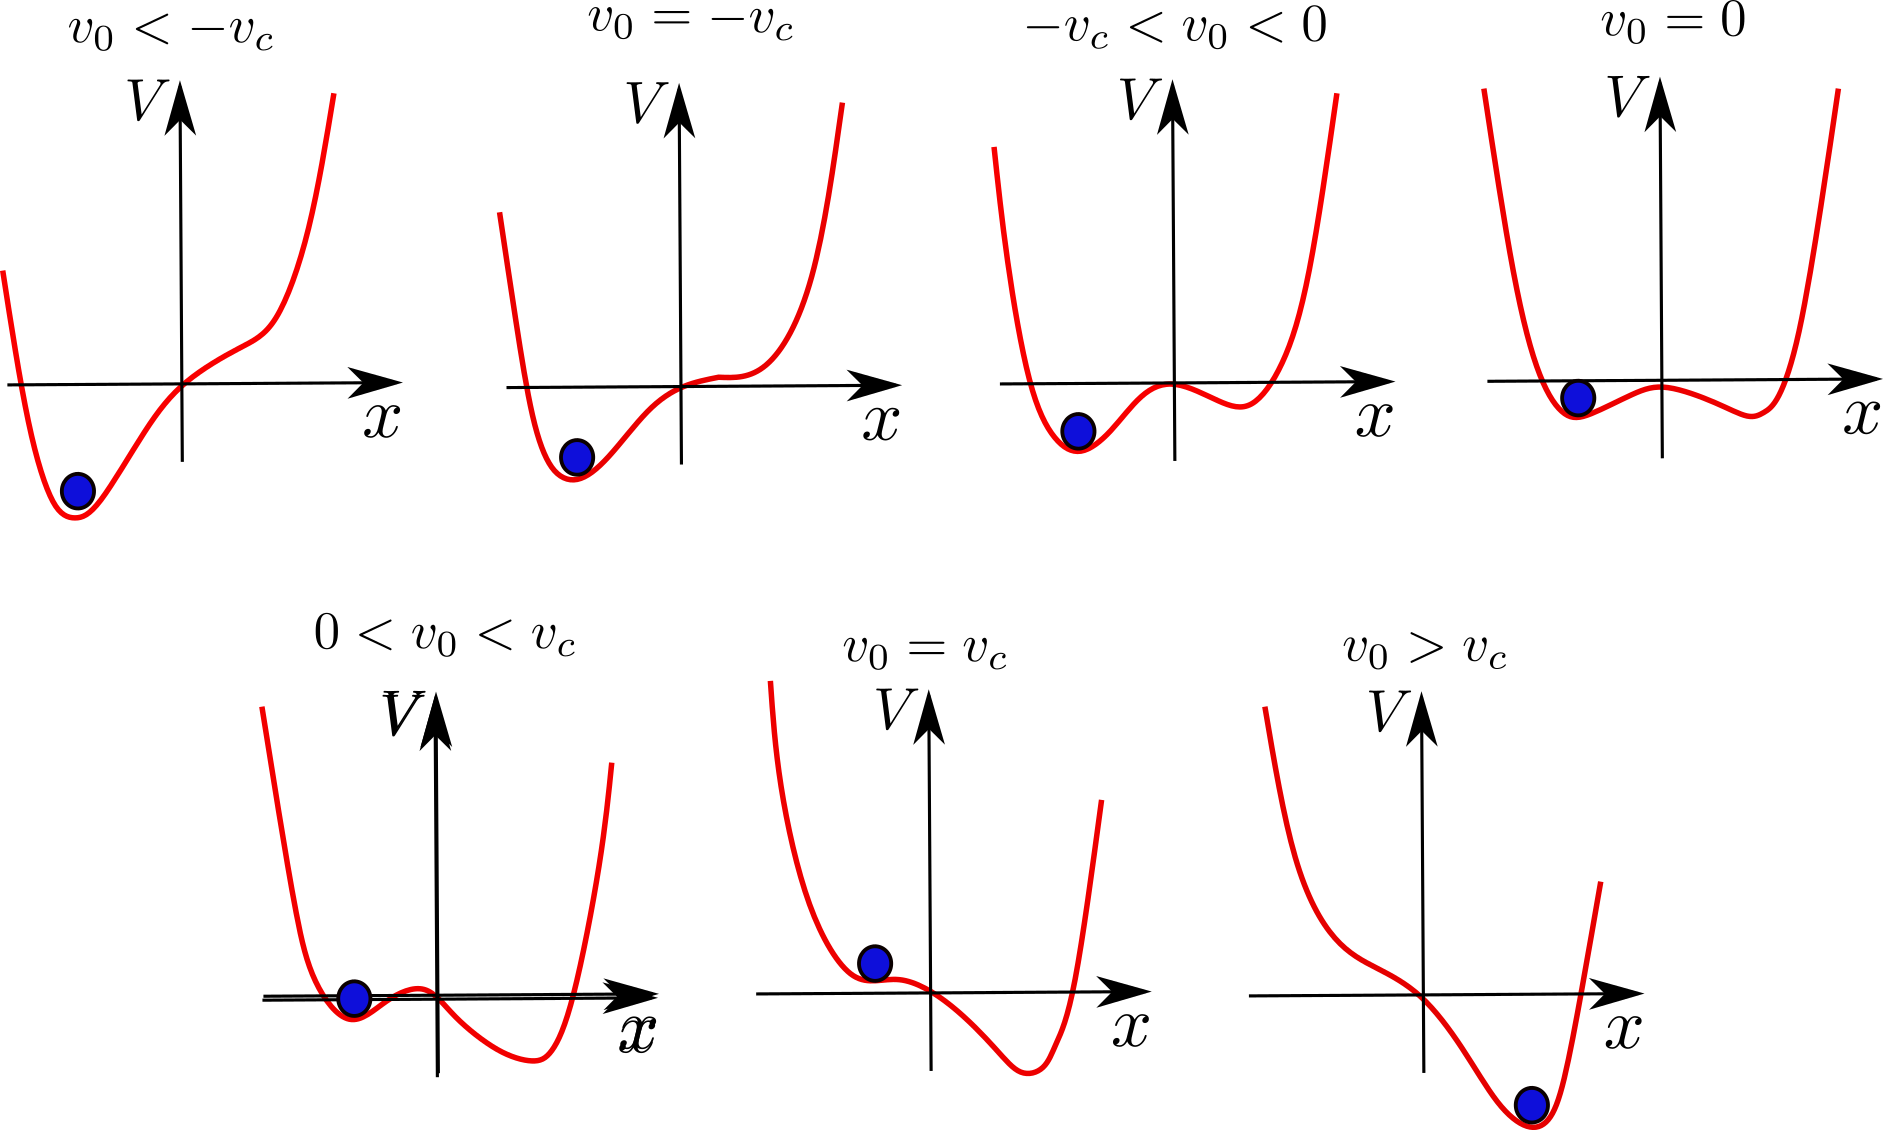
\includegraphics[width=5in]
{dynamical-sys/rolling-ball.png}
\caption{Interpretation of
critical velocity $v_c$
in terms of potential $V$.}
\label{fig-rolling ball}
\end{figure}


\section{Fixed Points in 2D Linear Systems}


In this section, we classify the fixed points for 
2D linear systems of the form

\beq
\dot{\vec{x}}=A\vec{x}
\eeq
where $\vec{x}\in\RR^2$
and $A\in\RR^{2\times 2}$.
But note
that if $A$ is invertible
(i.e., if $\det A \neq 0$),
this classification of
also applies to

\beq
\dot{\vec{x}}=A\vec{x} + \vec{c}
\eeq
where $\vec{c}\in\RR^2$,
 Indeed, 
 
\beq
\vec{\chi}=\vec{x}+A^{-1}\vec{c}
\implies 
\dot{\vec{\chi}}=A\vec{\chi}
\eeq

Let
\beq
\xymatrix{
\rvx \ar[d]\ar[dr]
& \rvy\ar[d]\ar[dl]
\\
\dot{\rvx} 
& \dot{\rvy}
}
\left\{
\begin{array}{l}
\dot{x} = a x + b y
\\
\dot{y}  = c x + d y
\end{array}
\right.
\eeq
where $a,b,c,d\in\RR$.

If we define
\beq
\vec{x} = \left[ 
\begin{array}{c}
x\\y
\end{array}
\right]
\;,\;\;
A = \left[
\begin{array}{cc}
a & b
\\
c & d
\end{array}
\right]
\eeq
then

\beq
\dot{\vec{x}} = A \vec{x}
\eeq


If we assume a solution of the form $\vec{x}=\vec{x_0}
e^{\lam t}$, then


\beq 
\vec{x}= \vec{x}_0 e^{\lam t}
\implies 
(A-\lam) \vec{x} =0\implies \det(A-\lam)=0
\eeq

\beq
 (a-\lam)(d-\lam)-bc = 0
\eeq
Hence

\beq
\lam^2 - 
\underbrace{(d + a)}_{=\tr(A)=\tau}\lam + 
\underbrace{(ad-bc)}_{=\det(A)=\delta}=0
\eeq

\beq
\lam =\lam_{\pm}=\frac{ \tau \pm \sqrt{\tau^2 - 4 \delta}}{2}
\eeq
If we define the discriminant $\Delta$ by

\beq
\Delta = \tau^2 - 4 \delta
\eeq
then

\beq
\lam = \lam_\pm =\frac{1}{2}(\tau\pm \sqrt{\Delta})
\eeq
The normalized eigenvectors $\vec{e}_\pm$ corresponding
to the eigenvalues $\lam_\pm$ satisfy

\beq 
A\vec{e}_\pm = \lam_{\pm}\vec{e}_\pm
\eeq


The most general solution 
of $\dot{\vec{x}}=A x$ is
\beq
\vec{x} = 
\Re\left[
\vec{e}_+ \alp_+ e^{\lam_+ t}
+
\vec{e}_- \alp_- e^{\lam_- t})
\right]
\label{eq-gen-sol-lode}
\eeq
where $\alp_\pm$ are complex constants. It can be easily checked that
Eq.(\ref{eq-gen-sol-lode}) satisfies $\dot{\vec{x}} = A \vec{x}$.

\subsection{Potential function}

Suppose the matrix $A$ can be diagonalized to $D=diag(\lam_1, \lam_2)$
via an orthogonal matrix $Q$.

\beq
A = Q^TDQ
\eeq
From $Q^TQ=QQ^T=1$, we get

\beq
\ddot{\vec{x}}=A\vec{x}
\implies
\underbrace{Q\ddot{\vec{x}}}_{\ddot{\vec{\xi}}}= D \underbrace{Q\vec{x}}_{\vec{\xi}}
\eeq
If $\vec{\xi} = (\xi_1, \xi_2)^T$,
then

\beq
\ddot{\xi}_i = \lam_i\xi_i\quad \text{for $i=1,2$}
\eeq
If we define

\beq
V=-\frac{1}{2}(\lam_1\xi^2_1 + \lam_2\xi^2_2)
\eeq
then

\beq
\lam_i\xi_i =-\partial_{\xi_i}V \quad \text{for $i=1,2$}
\eeq
Note that

\beq
V=
-\frac{1}{2}\vec{\xi}^TD\vec{\xi}=
=-\frac{1}{2}\vec{x}^TQ^TQ\vec{x}
\eeq
$\vec{x}^TQ^TQ\vec{x}$ is what is called a
{\bf quadratic form}.




\subsection{Classification of fixed points}

The {\bf fixed points} of the 2D system $\dot{\vec{x}}=A\vec{x}$ are 
the points $\vec{x}$ which satisfy:

\beq
0=\dot{\vec{x}}= A\vec{x}
\eeq
One can classify the types of fixed points by the behavior
of the streamlines in their vicinity.
The results are 
presented in Fig.\ref{fig-wiki-pp}.
To prove that figure, consider the following cases:


\begin{figure}[h!]
\centering
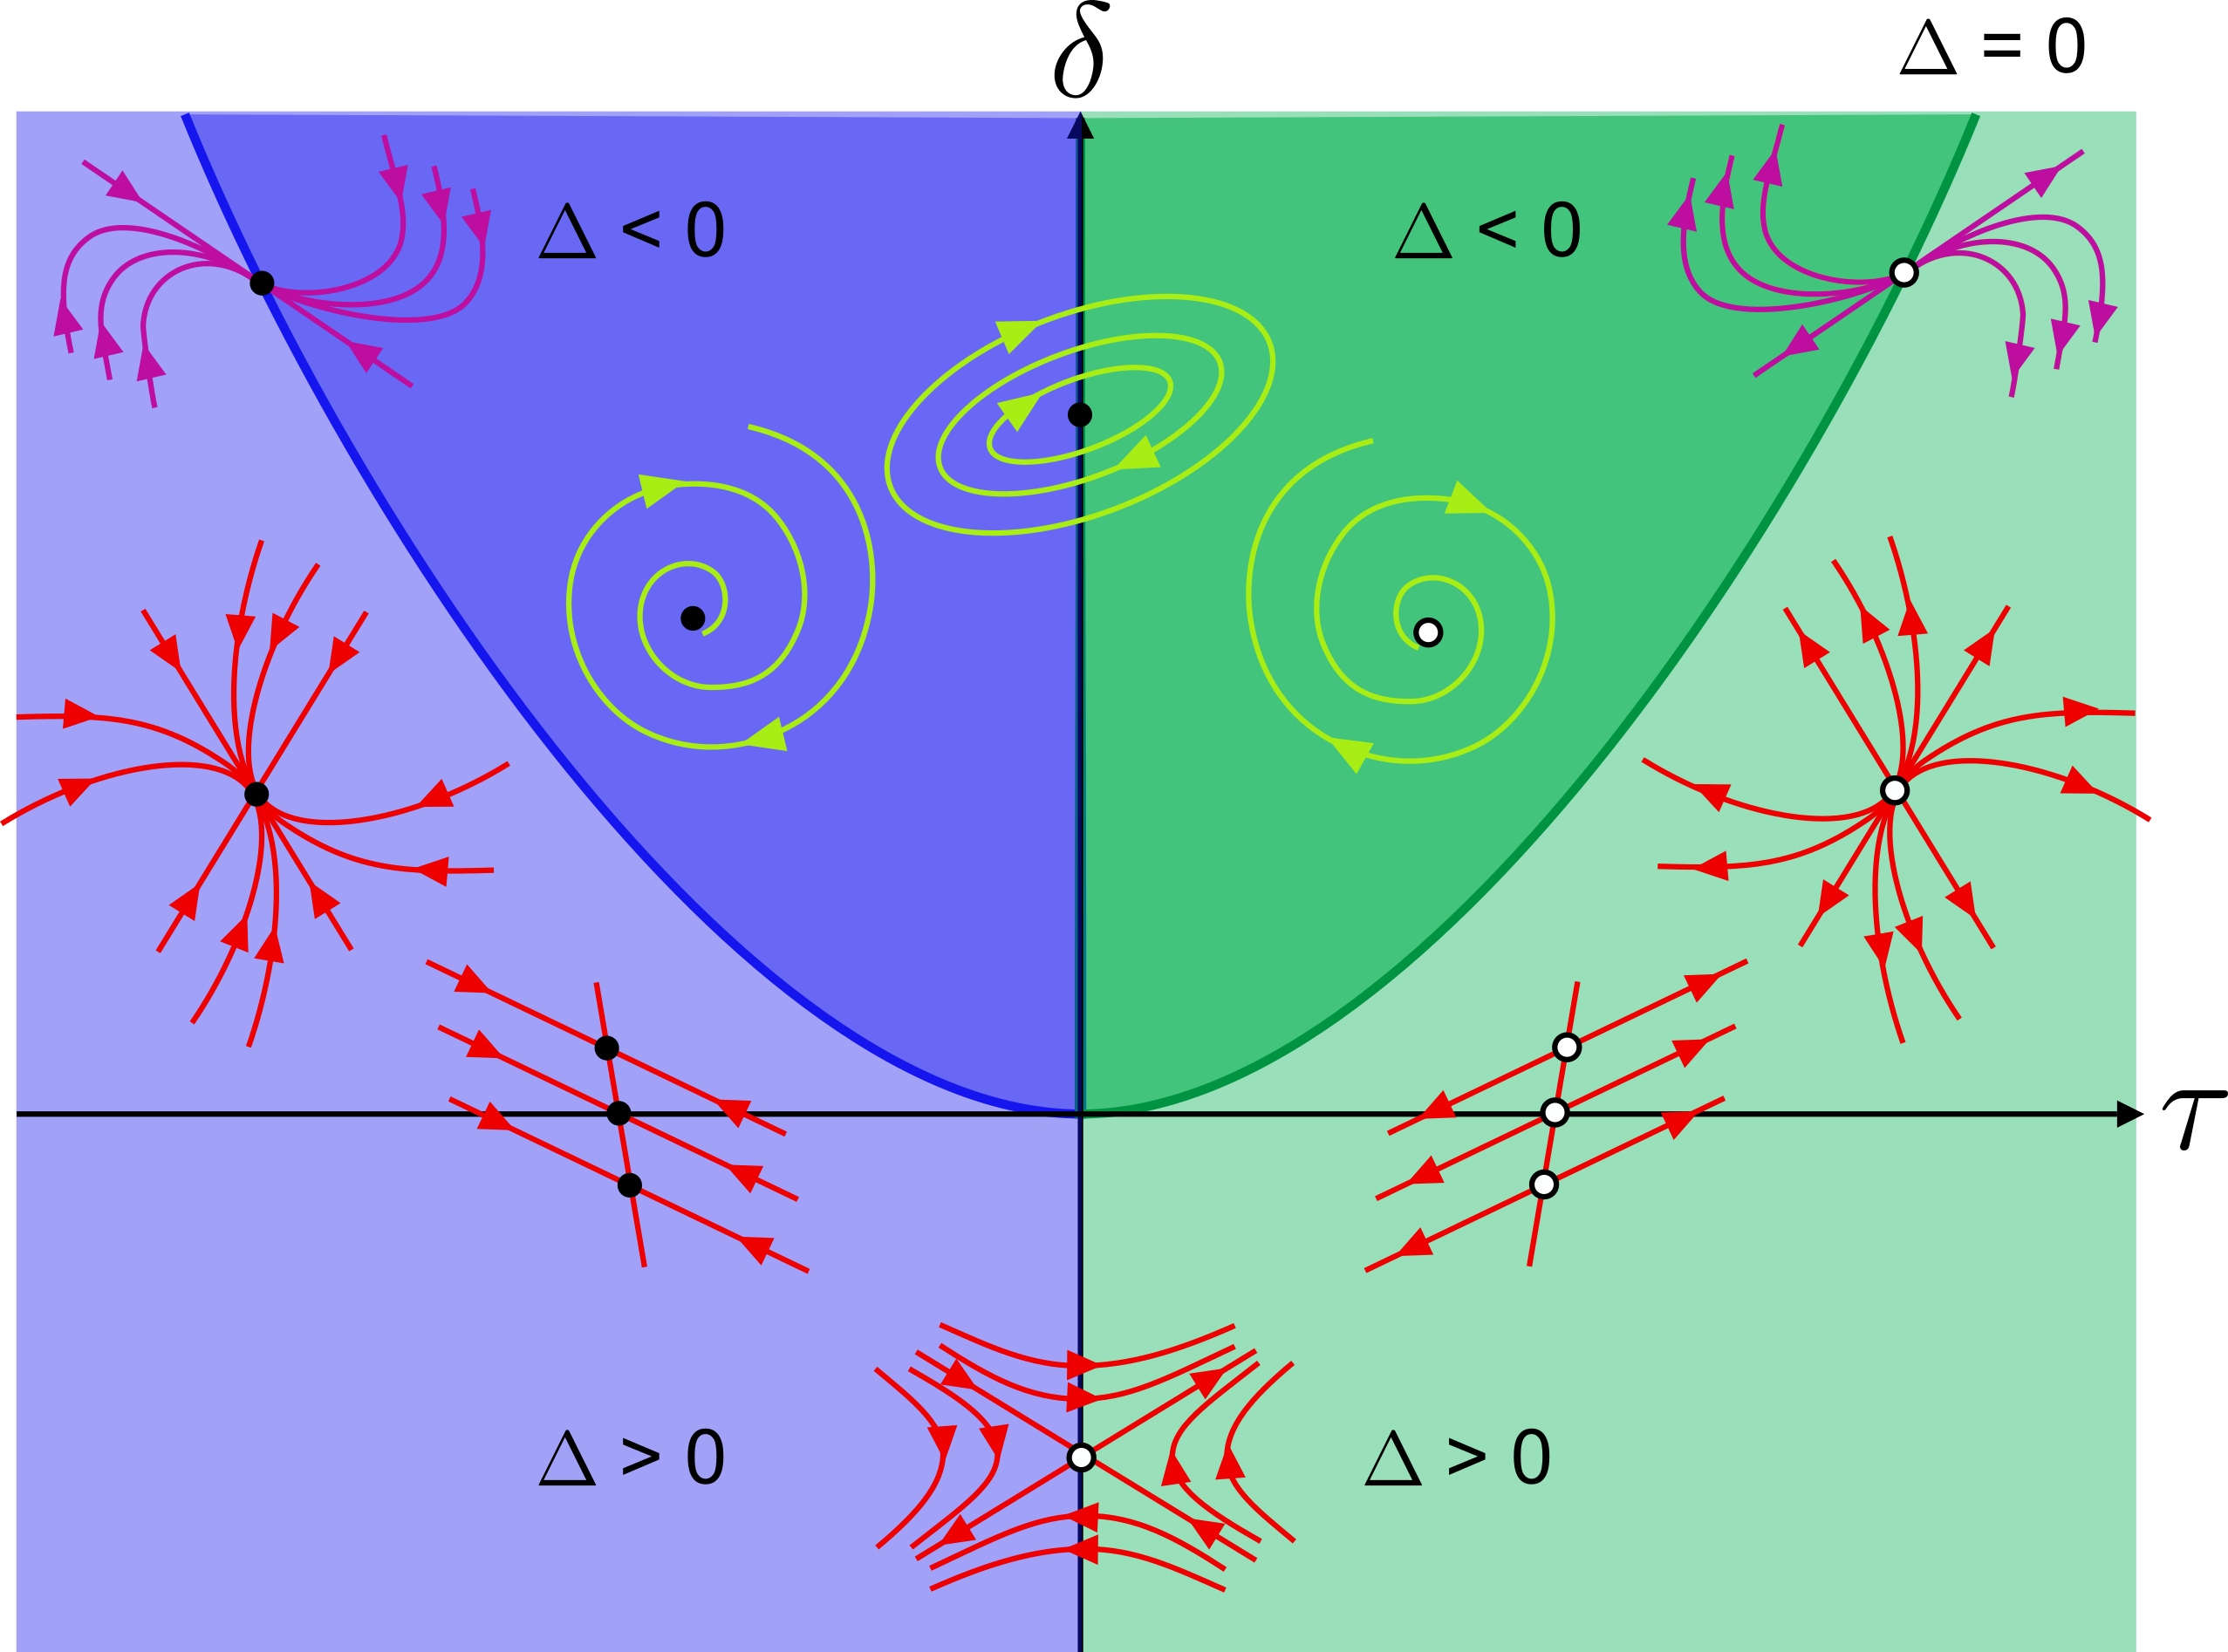
\includegraphics[width=3.8in]
{dynamical-sys/Phase_plane_nodes.png}
\caption{
$(\tau, \delta)$ plane
for $\dot{\vec{x}} = A \vec{x}$, where $A\in  \RR^{2\times 2}$ and  $\tau=\tr(A)$, $\delta=\det{A}$. This
figure  comes from Ref.\cite{wiki-phase-plane}}.
\label{fig-wiki-pp}
\end{figure}

\begin{itemize}
\item $\Delta < 0$:
complex eigenvalues,
oscillations (perhaps damped)
\begin{itemize}[\checkmark]
\item $\tau>0$: exponential growth, spiral out
\item $\tau=0$: {\bf center cycle}
\item $\tau<0$: exponential decay, spiral in
\end{itemize}


\item $\Delta = 0$:
real eigenvalues,
no oscillations. $\tau^2 = 4\delta$
\begin{itemize}[\checkmark]
\item $\tau>0$: exponential growth, source
\item $\tau=0$: $\lam=0$, $\vec{x}$ is constant in time.
\item $\tau<0$: exponential decay, sink
\end{itemize}

\item $\Delta > 0$:
real eigenvalues,
no oscillations 

\begin{itemize}[\checkmark]
\item both eigenvalues are negative: sink
\item both eigenvalues are positive: source
\item one eigenvalue ($\lam_-$) is negative 
and the other ($\lam_+$) is positive: saddlepoint. This 
includes case where $\tau=0$ so $\lam =\pm\frac{1}{2}\sqrt{\Delta}$.
\end{itemize}
\end{itemize}
\section{Bifurcations}

A {\bf bifurcation diagram}
(BD)
is a plot of $(\lam, x)$
where $\lam$ is
a parameter of the
system and $x$
is the value of one
of its  state
variables, assuming 
$\dot{x}=0$. A BD portrays
how one or more fixed points evolve
as $\lam$ changes, often 
bifurcating (i.e, splitting) into two fixed points.

We will  discuss 5 types of bifurcations.

\begin{enumerate}
\item {\bf saddlepoint bifurcation}

$x$ roots of
\beq
0=\dot{x}= v_0 + x^2
\eeq

\item{\bf transcritical bifurcation}

$x$ roots of
\beq
0=\dot{x}= \lam x -x^2
\eeq
\item {\bf supercritical pitchfork bifurcation} (\supercri)

$x$  roots of
\beq
0=\dot{x}=\lam x - x^3
\eeq
\item {\bf subcritical pitchfork bifurcation} (\subcri)

$x$ roots of 
\beq
0=\dot{x}=\lam x + x^3
\eeq

\item {\bf Hopf bifurcation}

$r$ roots of

\beq
0=\dot{r} = \mu_R r - r^3
\eeq
Note that a Hopf bifurcation is just a \supercri bifurcation with a change of notation.

\end{enumerate}




\subsection{Saddlepoint Bifurcation}

Fig.\ref{fig-bifur-saddle-point} gives plots of a saddlepoint
bifurcation.

The coordinates $(v_0, x)$ of the locus 
of fixed points is given by
\beq
0= \dot{x} = v_0 + x^2 \implies
 \TIL{x}_{\pm}=\pm \sqrt{-v_0}
 \eeq
 
 The type of
 fixed point can be 
 deduced from the second derivative
 of $V$.
 
 \beq
 V(x)= -v_0x -\frac{x^3}{3}
 \implies
 \partial^2_x V(x)= -2x
 \eeq
 
 \begin{figure}[h!]
 \centering
 \includegraphics[width=5in]
 {dynamical-sys/bifur-saddle-point.png}
 \caption{Saddle point bifurcation. $0= \dot{x} = v_0 + x^2$. 
 A sink and source collide and annihilate.
 This
 figure  comes from Ref.\cite{dynamical-fuchs}.}
 \label{fig-bifur-saddle-point}
 \end{figure}
 
\subsection{Transcritical Bifurcation}

Fig.\ref{fig-bifur-trans} gives plots of a transcritical
bifurcation.

The coordinates $(\lam, x)$ of the locus 
of fixed points is given by

\beq
0=\dot{x}=\lam x - x^2
\implies  \TIL{x}_1 =0\;\;\;
\TIL{x}_2 =\lam
\eeq

 The type of
 fixed point can be 
 deduced from the second derivative
 of $V$.
\beq
V(x) = -\lam\frac{x^2}{2}
+\frac{x^3}{3}
\implies
\partial^2_x V=-\lam + 2x
\eeq

\begin{figure}[h!]
 \centering
 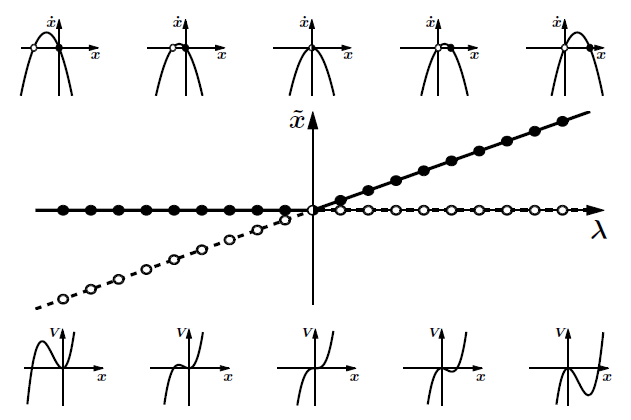
\includegraphics[width=5in]
 {dynamical-sys/bifur-trans.png}
 \caption{Transcritical bifurcation. $0=\dot{x}=\lam x - x^2$. 
 A sink and source collide and swap identities.
 This
 figure  comes from Ref.\cite{dynamical-fuchs}}.
 \label{fig-bifur-trans}
 \end{figure}
 
\subsection{Supercritical 
Pitchfork Bifurcation}
Fig.\ref{fig-bifur-super} gives plots of a \supercri
bifurcation.

The coordinates $(\lam, x)$ of the locus 
of fixed points is given by

\beq
0=\dot{x}=\lam x  - x^3
\implies \TIL{x}_1 =0
\;,\;\;
\TIL{x}_\pm = \pm \sqrt{\lam}
\eeq

 The type of
 fixed point can be 
 deduced from the second derivative
 of $V$.
\beq
V(x)=-\lam \frac{x^2}{2} 
+ \frac{x^4}{4}
\implies \partial^2_x V = -\lam + 3 x^2
\eeq

\begin{figure}[h!]
 \centering
 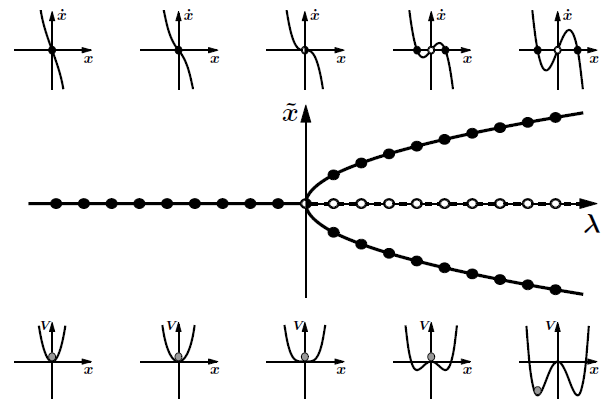
\includegraphics[width=5in]
 {dynamical-sys/bifur-super.png}
 \caption{\supercri bifurcation. 
 $0=\dot{x}=\lam x  - x^3$.
 A sink becomes a source and spawns two sinks
 in the process.
 The ball in this 
 figure exhibits
 the phenomenon called 
 {\bf spontaneous breaking of symmetry}. This
 figure  comes from Ref.\cite{dynamical-fuchs}.}
 \label{fig-bifur-super}
\end{figure}
 
\subsection{Subcritical
Pitchfork Bifurcation}

Fig.\ref{fig-bifur-sub} gives plots of a \subcri
bifurcation.

The coordinates $(\lam, x)$ of the locus 
of fixed points is given by


\beq
0=\dot{x}=\lam x  + x^3
\implies \TIL{x}_1 =0
\;,\;\;
\TIL{x}_\pm = \pm \sqrt{-\lam}
\eeq

 The type of
 fixed point can be 
 deduced from the second derivative
 of $V$.
 
\beq
V(x)=-\lam \frac{x^2}{2} 
- \frac{x^3}{3}
\implies \partial^2_x V = -\lam - 2x
\eeq

\begin{figure}[h!]
 \centering
 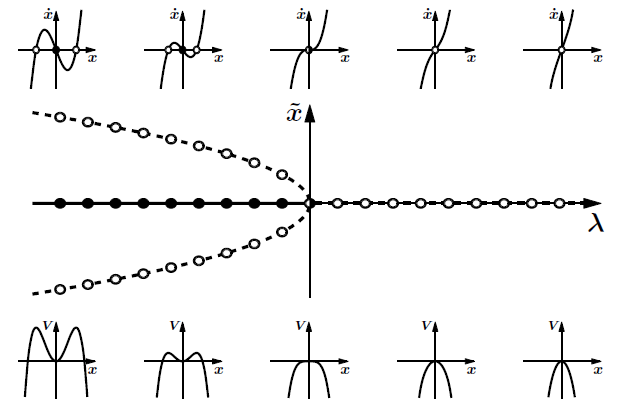
\includegraphics[width=5in]
 {dynamical-sys/bifur-sub.png}
 \caption{\subcri  bifurcation. $0=\dot{x}=\lam x  + x^3$. 
 A sink and two sources collide and spawn a source.
  This
 figure  comes from Ref.\cite{dynamical-fuchs}}.
 \label{fig-bifur-sub}
 \end{figure}

\subsection{Hopf Bifurcation}

Consider the system
\beq
\xymatrix@R=.5pc{
&\vec{\rvx}\ar[dd]
\ar[dl]
\\
|\vec{\rvx}|^2\ar[dr]
|\redminus
\\
&\dot{\vec{\rvx}}
}
\quad\quad
\left\{
\dot{\vec{x}}=\left[A -|\vec{x}|^2\right]\vec{x}
\right.
\label{eq-hopf-vector}
\eeq
where

\beq 
\vec{x}=
\left[
\begin{array}{c}
x\\ y
\end{array}
\right]
\;,\;\;
A =
\left[
\begin{array}{cc}
\mu_R
& -\mu_I
\\
\mu_I & \mu_R
\end{array}
\right]
\eeq
and $x, y, \mu_R, \mu_I\in\RR$.

Let $\mu = \mu_R + i\mu_I$. Note that in the linear approximation which is valid for $|\vec{x}|<<1$, we have
$\dot{\vec{x}}=A\vec{x}$.
This is satisfied by $\vec{x}=\vec{x}_0 e^{At}$.
The eigenvalues of $A$ are
$\mu, \mu^*$  because

\beqa
\det(A-\lam)
&=&(\mu_R-\lam
)(\mu_R-\lam) + \mu_I^2
\\
&=&
(\lam - \mu_R - i \mu_I)
(\lam - \mu_R + i \mu_I)
\\
&=&
(\lam -\mu)(\lam -\mu^*)
\eeqa


Let

\beq 
\calc(\vec{x}) = x+ iy
\eeq
for any $\vec{x}=
(x,y)^T\in\RR^2$. 


If 
$ z= x + iy$ and 
$\mu = \mu_R + i\mu_I$,
then

\beqa
\mu z&=&
(\mu_R + i\mu_I)(x+iy)
\\
&=&
(\mu_R x -\mu_I y)
+i(\mu_I x + \mu_R y)
\\
&=&
(A\vec{x})_0 + i (A\vec{x})_1
\\
&=& \calc(A\vec{x})
\eeqa
Applying $\calc()$
to both sides of Eq.(\ref{eq-hopf-vector}), we get

\beq
\dot{z} = (\mu - |z|^2) z
\label{eq-hopf-complex}
\eeq

In polar coordinates, with $z= r^{i\theta}$,
Eq.(\ref{eq-hopf-complex}) reduces to

\beq
(\dot{r} + i\dot{\theta}r)e^{i\theta}=
(\mu - r^2)r e^{i\theta}
\eeq
Hence, 
\beq
\left\{
\begin{array}{l}
\dot{r}= (\mu_R - r^2)r
\\
\dot{\theta}=\mu_I
\end{array}
\right.
\eeq
Note that in polar coordinates,
the two ODE decouple and
the second one is trivial to
solve.

\beq
\theta = \mu_I  t
\eeq
Note also that the first ODE is the same ODE that we considered 
for a
\supercri bifurcation Fig.\ref{fig-bifur-super}.

In $(r, V)$ space,
for $\mu_R<0$, 
$V$ is a $U$ shaped potential
 with a minimum at $r=0$.
 For $\mu_R>0$, $V$ is a
W shaped potential
with two minima at $r=\pm \sqrt{\mu_R}$.

In $((x,y), V)$ space, for $\mu_R<0$,
$V$ is a
\qt{bowl} shaped potential
 with a minimum at $r=0$.
For $\mu_R>0$, $V$ is a 
\qt{Mexican hat}
shaped potential whose minima
form a circle of radius $r=\sqrt{\mu_R}$. 

%\begin{figure}[h!]
%\centering
%\includegraphics[width=5in]
%{dynamical-sys/hopf-evas.png}
%\caption{Eigenvalues of $A-|\vec{x}(t)|^2$ for Hopf
%Eq.(\ref{eq-hopf-vector}).}
%\label{fig-hopf}
%\end{figure}

\section{Hysteresis}

\begin{figure}[h!]
 \centering
 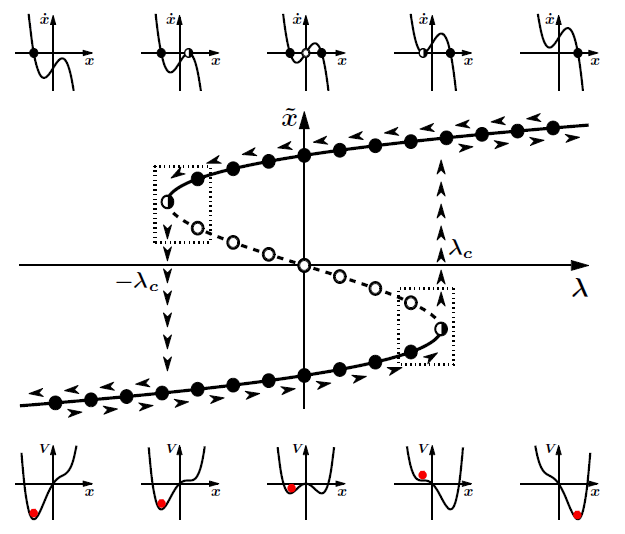
\includegraphics[width=5in]
 {dynamical-sys/hysteresis-2-saddle-points.png}
 \caption{Hysteresis arises in systems with  2 saddlepoints from which the system \qt{escapes}. The red ball rolling downhill in the $(x,V)$
 plots represents
 the fast transitions (escapes) of hysteresis. This
 figure  comes from Ref.\cite{dynamical-fuchs}.}
 \label{fig-hysteresis-2-saddle-point}
 \end{figure}
 
 As show in Fig.\ref{fig-hysteresis-2-saddle-point}, {\bf hysteresis}
 arises in systems with 2 saddlepoints, S1, S2. In the $(\lam, x)$ plot,
 as the parameter $\lam$ is 
 cycled between $-\lam_c$ and $\lam_c$,
 the system travels along a
 line of increasingly weak attractors which turn into  saddlepoint S1, at which point the system jumps to a string of increasingly weak attractors
 that turn into saddlepoint S2.

 \begin{figure}[h!]
\centering
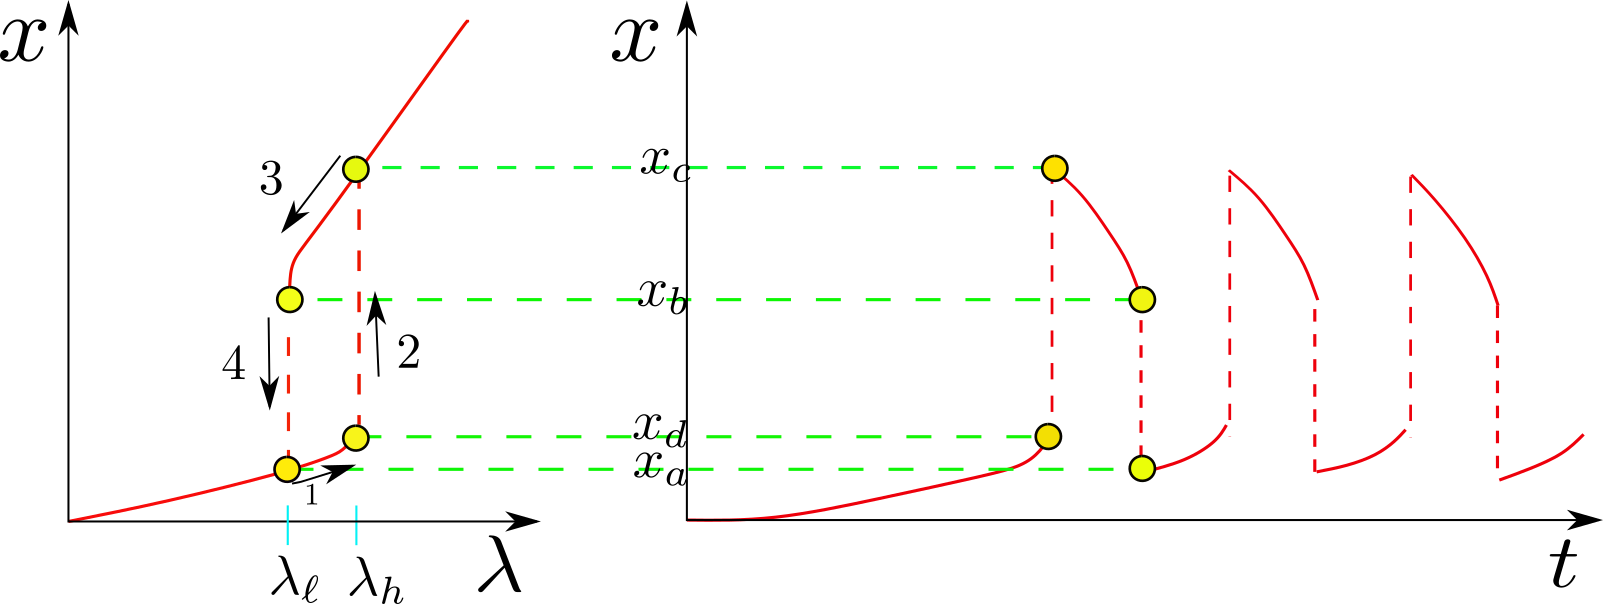
\includegraphics[width=5in]
{dynamical-sys/hysteresis.png}
\caption{In hysteresis,
as we cycle 
$\lam$ between $\lam_\ell$ and $\lam_h$, the $x(t)$ 
produced is a
train of pulses.}
\label{fig-hysteresis}
\end{figure}

 As shown in Fig.\ref{fig-hysteresis},
 if we cycle the parameter $\lam$
 between $-\lam_c$ and 
 $\lam_c$, the $x(t)$ produced is a
 train of pulses
 which can be used as a clock.
 


\section{Limit cycles}

A {\bf limit cycle} is an \qt{isolated} closed trajectory with no saddlepoints
 in it. There are four types of limit cycles, depending on whether their surface attracts or repels inside and outside.
 These 4 types are portrayed  in Fig.\ref{fig-limit-cycles}. Of these 4 types, only one type
 is truly stable,  the one whose surface attracts both inside and outside (i.e., type $(A)A$).
 
 Limit cycles are quite different from the {\bf center cycles} that we introduced under linear systems.
 Limit cycles did not arise in our classification of fixed points for linear systems, so they are exclusively non-linear phenomena.\footnote{
 In 2D, $V$ is shaped like a bowl for the center cycles of a linear system, but
 shaped like a
 Mexican hat for the limit cycles
 of a non-linear system.} Furthermore, 
 the surface of a center cycle neither attracts
 nor repels trajectories either inside
 or outside. For any center cycle, 
 there is another infinitesimally bigger
 center cycle  running parallel to it.
 This is not the case for limit cycles.
 In fact, that is what we mean when we say  
 that limit cycles are 
 \qt{isolated}. The cycle produced 
 by a Hopf bifurcation is a stable limit cycle, not a center cycle.
 

\begin{figure}[h!]
\centering
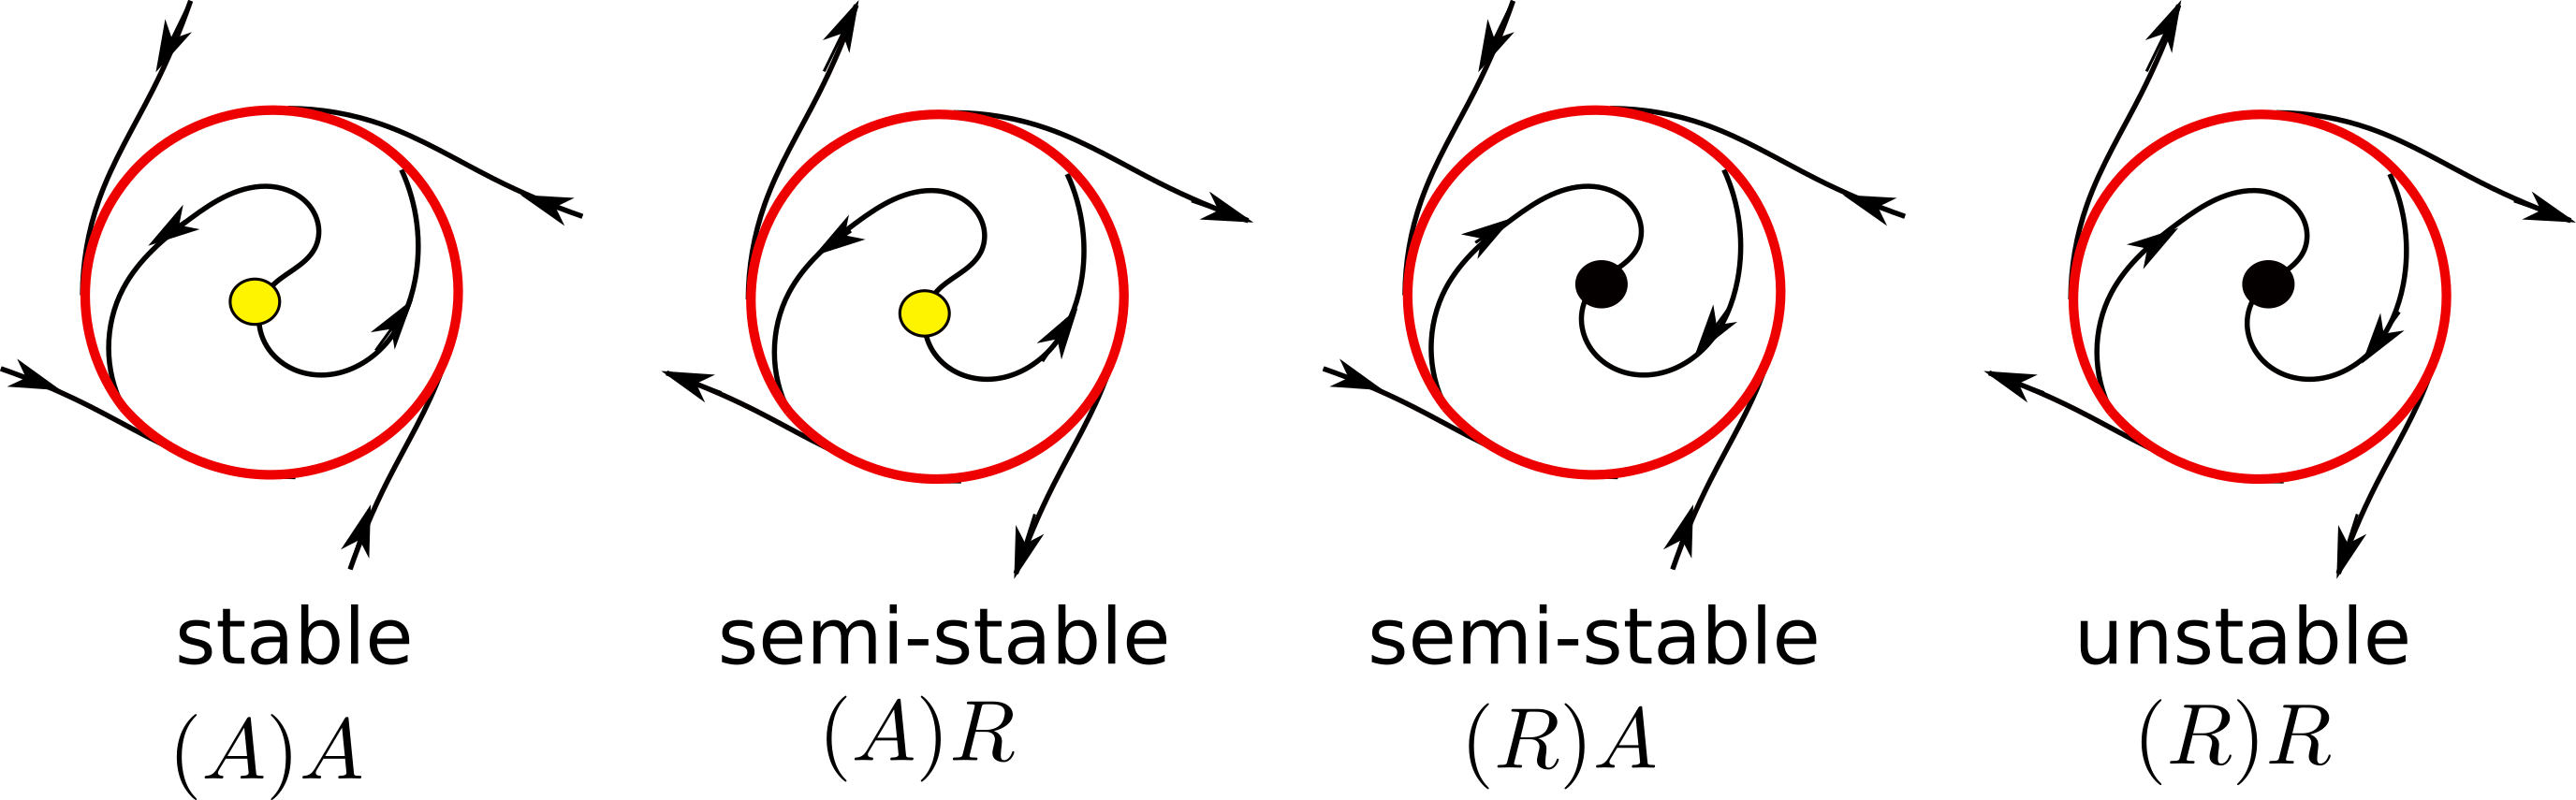
\includegraphics[width=4in]
{dynamical-sys/limit-cycles.png}
\caption{The four types of limit cycles. If the 
surface of the cycle attracts inside and repels outside,
we call it an $(A)R$. The names of the other types
are defined similarly. }
\label{fig-limit-cycles}
\end{figure}

\section{Homoclinic and Heteroclinic orbits}

As illustrated by Fig.\ref{fig-homo-hetero-clinic}, 
a {\bf homoclinic (or heteroclinic) orbit}  is a closed trajectory which contains a one saddlepoint if homoclinic (or two if heteroclinic), and for which the flow runs
parallel to the surface, both inside and outside. 
Homoclinic and heteroclinic orbits have a parallel
flow pattern inside and outside, just like center cycles, but,
unlike center cycles,  they contain saddle points. 
A trajectory can enter or exit the orbit through any of the saddlepoints of the orbit.

\begin{figure}[h!]
\centering
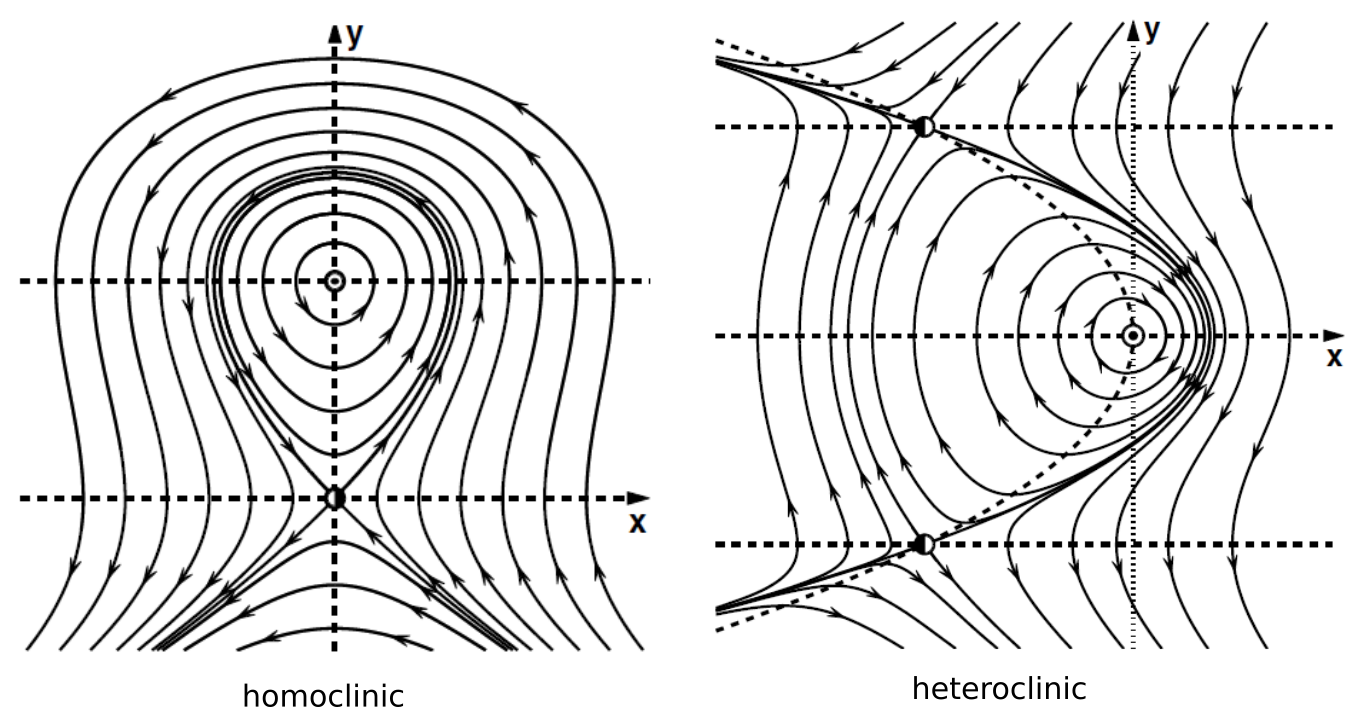
\includegraphics[width=6in]
{dynamical-sys/homo-hetero-clinic.png}
\caption{Homoclinic and Heteroclinic orbits.
These two
 figures  come from Ref.\cite{dynamical-fuchs}.}
\label{fig-homo-hetero-clinic}
\end{figure}


\section{Oscillators}

\subsection{Linear oscillator}

The position $x$ 
at time $t$ of a particle of mass $m$, subjected 
to a spring force $-k x$,
a 
damping force $-2\gamma m \dot{x}$
($\gamma$ is called the {\bf damping coefficient})
and driven by a force $F_0cos(\omega t)$,
satisfies Newton's equation given by

\beq
m\ddot{x} =- 2\gamma m \dot{x} - 
k x + F_0\cos(\omega t)
\label{eq-ho}
\eeq
If we define the {\bf natural frequency}  $\omega_0$ by

\beq
\omega_0 = \sqrt{\frac{k}{m}}
\eeq
then this equation can be transformed into two 1st order ODE

\beq
\xymatrix@C=2pc{
\rvx \ar@/_1pc/[dr]|\redminus
&\rvv\ar[d]|\redminus
\ar@/_1pc/[dl]|\redplus
\\
\dot{\rvx}
&\dot{\rvv}&\ar[l]
}
\quad\quad
\left\{
\begin{array}{l}
\dot{x} = v
\\
\dot{v} = -2\gamma v -\omega^2_0 x - \frac{F_0}{m} \cos(\omega t)
\end{array}
\right.
\eeq 

The most general solution of Eq.(\ref{eq-ho})
is
\beq
x = x_h + x_p
\eeq
where
$x_h$ is the {\bf homogeneous solution} 
(independent of $F_0$) and $x_p$  is the {\bf particular solution}
(dependent on $F_0$). Explicit expressions for each will
be given next.

\begin{claim}\label{cl-ho-solutions}
For the harmonic oscillator Eq.(\ref{eq-ho}), the homogeneous solution $x_h$
is

\begin{itemize}

\item if $\gamma < \omega_0$ (underdamping)

\beq
\boxed{x_h =\Re(A_he^{-\gamma t +i(\TIL{\omega}_0 t +\delta)})}
\eeq
where $\TIL{\omega}_0=\sqrt{\omega_0^2 -\gamma^2}$
and $A_h, \delta\in\RR$

\item if $\gamma = \omega_0$ (critical damping)

\beq
\boxed{x_h = A_h e^{-\gamma t}[1 +  bt]}
\eeq
for some $A_h, b\in\RR$.

\item if  $\gamma > \omega_0$ (overdamping)

\beq
\boxed{x_h =A_h e^{-\gamma_+ t} + B_h e^{-\gamma_- t}}
\eeq
where $\gamma_\pm =\gamma \pm  \sqrt{\gamma^2 -\omega_0^2}$,
and $A_h, B_h \in\RR$.


\end{itemize}




\end{claim}
\proof

We find the homogeneous solution by setting $F_0$ 
to zero in Eq.(\ref{eq-ho}).
Assume 

\beq
x_h = \Re\left(A_he^{i\delta}e^{\lam t}\right)
\label{eq-ho-homog}
\eeq
where $A_h, \delta\in \RR$ and $\lam\in \CC$. Then

\beq
A_h(\lam^2 + 2\gamma\lam +\omega_0^2) = 0
\eeq
so

\beqa
\lam &=&\frac{1}{2}(-2\gamma \pm \sqrt{4\gamma^2-4\omega_0^2}
\\
&=&
-\gamma\pm i \underbrace{\sqrt{\omega_0^2-\gamma^2}}_{\TIL{\omega}_0}
\eeqa
Substituting this value
of $\lam$ into 
Eq.(\ref{eq-ho-homog}),
we finally get

\beq
x_h =\Re(A_h e^{-\gamma t +i(\TIL{\omega}_0 t +\delta)})
\eeq

When $\omega_0^2 = \gamma^2 +\epsilon^2$
where $0<\epsilon <<1$, this reduces  to

\beqa
x_h &=& A_h e^{-\gamma t}\cos(\epsilon t +\delta)
\\
&=&
A_h e^{-\gamma t}[ \cos(\epsilon t)\cos(\delta)-
\sin(\epsilon t)\sin(\delta)]
\\
&\approx &
\underbrace{A_h\cos(\delta)}_{A'_h}e^{-\gamma t}[1 -  \tan(\delta) \epsilon t]
\eeqa
\qed

The most interesting damped case is often assumed; namely, 
underdamping
$0\leq \gamma< \omega_0$

Claim \ref{cl-ho-solutions}
assumes $\gamma\geq 0$. If $\gamma <0$, we get
an oscillation with exponentially increasing amplitude.
This is no longer damping, although it is sometimes 
referred to as {\bf negative damping}. Negatively damped 
oscillators are also often called
{\bf unstable}, {\bf anti-damped}, {\bf self-exciting},
{\bf self-amplifying} or {\bf exponentially growing}
oscillators. They arise frequently in Nature (in Biology, Chemistry, Physics) in systems with {\bf positive feedback}.
Of course, the amplitude cannot grow exponentially 
for very long time because any real system has finite resources
and that will cap the growth.

\begin{claim}
For the harmonic oscillator Eq.(\ref{eq-ho}), the particular
solution $x_p$ is

\beq
\boxed{x_p =A\cos(\omega t-\delta)}
\eeq
where

\beq
\boxed{A = \frac{F_0}{m}\frac{1}{
\sqrt{(\omega_0^2-\omega^2)^2 + (2\omega\gamma)^2}}}
\eeq
and

\beq
\boxed{\tan\delta
=
\frac
{2\omega \gamma}
{\omega^2_0 -\omega^2}}
\eeq

\end{claim}
\proof

If we substitute 
\beqa
x_p &=&A{\cos(\omega t-\delta)}
\\
&=&
\frac{A}{2}(e^{i(\omega t -\delta)}+ e^{-i(\omega t -\delta)})
\eeqa
into Eq.(\ref{eq-ho}), we get\footnote{c.c. means complex conjugate. $z + c.c. = z+z  ^*$.
This notation is especially useful when  $z$ is a long expression.}

\beq 
\frac{A}{2}e^{i(\omega t -\delta)}(
-\omega^2  + i2\omega \gamma +\omega_0^2) + c.c.=
\frac{F_0}{2m}(e^{i\omega t}) + c.c.
\eeq
Hence,

\beq
Ae^{-i\delta t}\underbrace{(
-\omega^2  + i2\omega \gamma +\omega_0^2) }_{z}
=\frac{F_0}{m}
\eeq
Therefore,

\beqa
A &=& \frac{F_0}{m}\frac{1}{
|z|}
\\
&=& \frac{F_0}{m}\frac{1}{
\sqrt{(\omega_0^2-\omega^2)^2 + (2\omega\gamma)^2}}
\eeqa
Furthermore

\beqa
e^{-i\delta t} \frac{z}{|z|}=1
\eeqa
so

\beq
\delta =\angle \left( \frac{z}{|z|}\right)
\eeq
which means

\beqa
\tan\delta
&=& \frac{z_I}{z_R}
\\
&=&
\frac
{2\omega \gamma}
{\omega^2_0 -\omega^2}
\eeqa
\qed





The {\bf power spectrum} of $x(t)$ is defined as

\beq
S(\nu)=|\TIL{x}(\nu)|^2
\eeq
where 

\beq
\TIL{x}(\nu) =\calf[x(t)]
=\int_{-\infty}^{\infty}dt\;
\; e^{i\nu t}x(t)
\eeq

\begin{claim}
The power spectrum for the harmonic oscillator Eq.(\ref{eq-ho})
is as follows:

\beq
\boxed{S(\nu) = |\TIL x(\nu)|^2=
\frac{A^2}{4}
\left[
\frac{1}{\gamma^2 + (\nu-\TIL{\omega}_0)^2}
+
\frac{1}{\gamma^2 + (\nu+\TIL{\omega}_0)^2}
\right]}
\label{eq-spectrum-ho}
\eeq
\end{claim}
\proof

\beqa
\TIL{x}(\nu)  &=& \calf[A e^{-\gamma t}\cos(\TIL{\omega}_0 t -\delta)]
\\
&=&\calf\left[
\frac{A e^{-\gamma t}}{2}(e^{i(\TIL{\omega}_0 t -\delta)}
+ e^{-i(\TIL{\omega}_0 t -\delta)})
\right]
\\
&=&
\frac{A }{2} \left(
\underbrace{\frac{e^{-i\delta}}{-\gamma + i(\nu + \TIL{\omega}_0)}}_{z_+}
 + 
 \underbrace{\frac{e^{+i\delta}}{-\gamma + i(\nu - \TIL{\omega}_0)}}_{z_-} \right)
\eeqa
Thus,

\beq
S(\nu)=\frac{A^2}{4}
[|z_-|^2 + |z_+|^2
+ 2\Re(z_- z_+^*)]
\eeq
The cross term $2\Re(z_- z_+^*)$
is usually neglected because
it is overpowered by the two terms $|z_\pm|^2$
in the regions of most interest,
namely in the vicinity of the two peaks  at $\nu=\pm\TIL{\omega}_0$.
Hence,

\beq
S(\nu)\approx 
\frac{A^2}{4}
\left[
\frac{1}{\gamma^2 + (\nu-\TIL{\omega}_0)^2}
+
\frac{1}{\gamma^2 + (\nu+\TIL{\omega}_0)^2}
\right]
\eeq
\qed

The {\bf Q factor} (quality factor) of a damped harmonic oscillator is defined as

\beq
Q= \frac{\omega_0}{2\gamma}
\eeq
If $\norm{a(t)}=\max_t|a(t)|$, then

\beq
\frac{\norm{\omega_0^2 x(t)}}{\norm{ 2\gamma \dot{x}(t)}}
\approx
\frac{\omega_0^2 A \norm{\cos(\omega_0 t-\delta)}}{2\gamma \omega_0A \norm{-\sin(\omega_0 t-\delta)}}
=
Q
\eeq


\subsection{Nonlinear Oscillators}
The linear harmonic oscillator
Eq.(\ref{eq-ho})
considered in the previous
section can be
generalized to
 
\beq
\ddot{x} + 2\gamma \dot{x} + \omega_0^2 x + \calf_2(x, \dot{x})  + \calf_3(x, \dot{x})=0
\eeq
where $\calf_2$ and $\calf_3$ are sums of terms  that are second and third order in $x$ ($x\dot{x}^2$ is
considered to be a third order in $x$ term).

Notice that solutions $x(t)$
of the linear oscillator
Eq.(\ref{eq-ho})
continue to be solutions if $x\rarrow -x$, except their initial conditions change because $-e^{i\omega t}= e^{i(\omega t +\pi)})$.
This property is called {\bf
reflection invariance} (RI)
because it manifests itself in the property that the equation
of motion Eq.(\ref{eq-ho})
is invariant under the
transformation $x\rarrow -x$.
To reduce the number of possibilities for $\calf_2$ and
$\calf_3$ terms, we
consider only terms that 
preserve RI by being odd under
$x\rarrow -x$.
This rules out all $\calf_2$ terms
and leaves only 4 possible terms for $\calf_3$:

\beq 
\calf_3 = \underbrace{
\underbrace{V x^2\dot{x}}_{\text{Van der Pol term}}
+
\underbrace{R \dot{x}^3}_{\text{Raleigh term}}
}_{\text{V-R hybrid term (odd in $\dot{x}$)}}
+ \underbrace{ C x(\dot{x})^2  + 
\underbrace{D x^3}_{\text{Duffing term}}
}_{\text{even in $\dot{x}$}}
\eeq

In particular,
we wish to consider the {\bf V-R hybrid model}
whose equation of motion is

\beq
\ddot{x} + \underbrace{(2\gamma + V x^2 + R \dot{x}^2 )}_{2\TIL{\gamma}}
\dot{x} +\omega_0^2 x=0
\eeq

Note that the Van der Pol equation is usually written as
(see Ref.\cite{wiki-van-der-pol}):

\beq \ddot{x}  -\mu(1-x^2)\dot{x}+ x=0
\quad (\text
 {$2\gamma = -\mu$, $V=\mu$
$\omega^2_0=1$})
\eeq
The reason for
assuming this special case is that it leads to a 
stable limit cycle for $\mu>0$. 

\begin{claim}
 $\gamma<0$ and $V>0$ are necessary to get a 
 stable limit cycle
 in the Van der Pol equation.
 By the same argument, $\gamma<0$ and $R>0$ are necessary
 for a stable limit cycle in the Raleigh oscillator.
 \end{claim} 
 \proof
 
The effective damping is
\beq
2\TIL{\gamma}= 2\gamma + Vx^2
\eeq
\begin{itemize}
\item
To get $\TIL{\gamma}<0$   when $|x|\approx 0$ requires $\gamma<0$. 
\item 
To get $\TIL{\gamma}>0$ when $|x|\rarrow \infty$
requires $V>0$
\end{itemize}
\qed



\begin{figure}[h!]
\centering
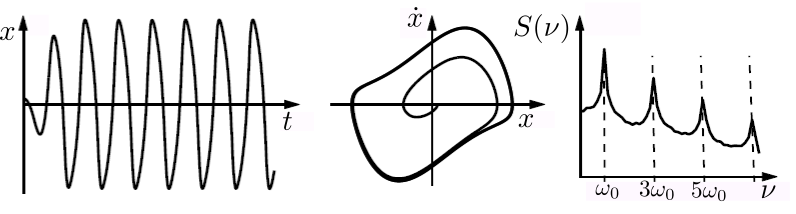
\includegraphics[width=5in]
{dynamical-sys/van-der-pol-term.png}
\caption{Van der Pol oscillator. This
 figure  comes from Ref.\cite{dynamical-fuchs}.}
\label{fig-van-der-pol-term}
\end{figure}

\begin{figure}[h!]
\centering
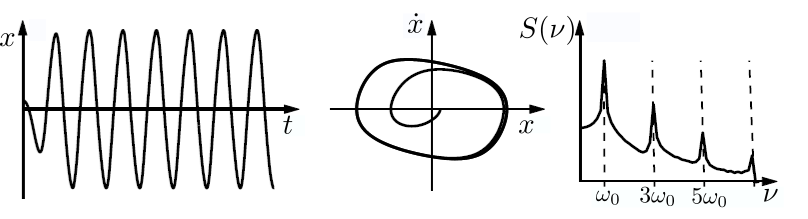
\includegraphics[width=5in]
{dynamical-sys/raleigh-term.png}
\caption{Raleigh oscillator. This
 figure  comes from Ref.\cite{dynamical-fuchs}.}
\label{fig-raleigh-term}
\end{figure}

\begin{figure}[h!]
\centering
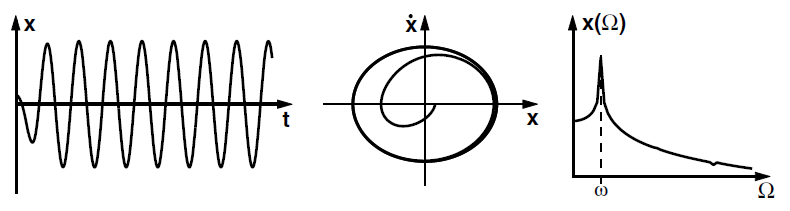
\includegraphics[width=5in]
{dynamical-sys/hybrid-term.png}
\caption{V-R hybrid oscillator. This
 figure  comes from Ref.\cite{dynamical-fuchs}.}
\label{fig-hybrid-term}
\end{figure}


Figs.\ref{fig-van-der-pol-term},
\ref{fig-raleigh-term}
and \ref{fig-hybrid-term}
show typical
$x(t)$ traces, $(x, \dot{x})$
PPs and spectra $S(\nu)$
for the Van der Pol ($V\neq 0,R=0$), Raleigh
($V=0$, $R\neq 0$) and hybrid  ($V\neq 0,R\neq 0$)
oscillators.
Note that all 3
have a peak at 
the {\bf fundamental frequency} $\omega_0$.
The V and R oscillators also have peaks   
at
odd {\bf higher harmonics} ($3\omega_0, 5\omega_0$, etc.)
whereas those higher harmonic peaks are
suppressed in a hybrid oscillator.
Of course, the linear harmonic oscillator
 spectrum has no higher harmonic peaks either.
But the $\omega_0$ dependence of
the peak value of the power spectrum of the V-R hybrid oscillator
has a desirable property which the linear oscillator doesn't have. Indeed, note the following claim. 


\begin{figure}[h!]
\centering
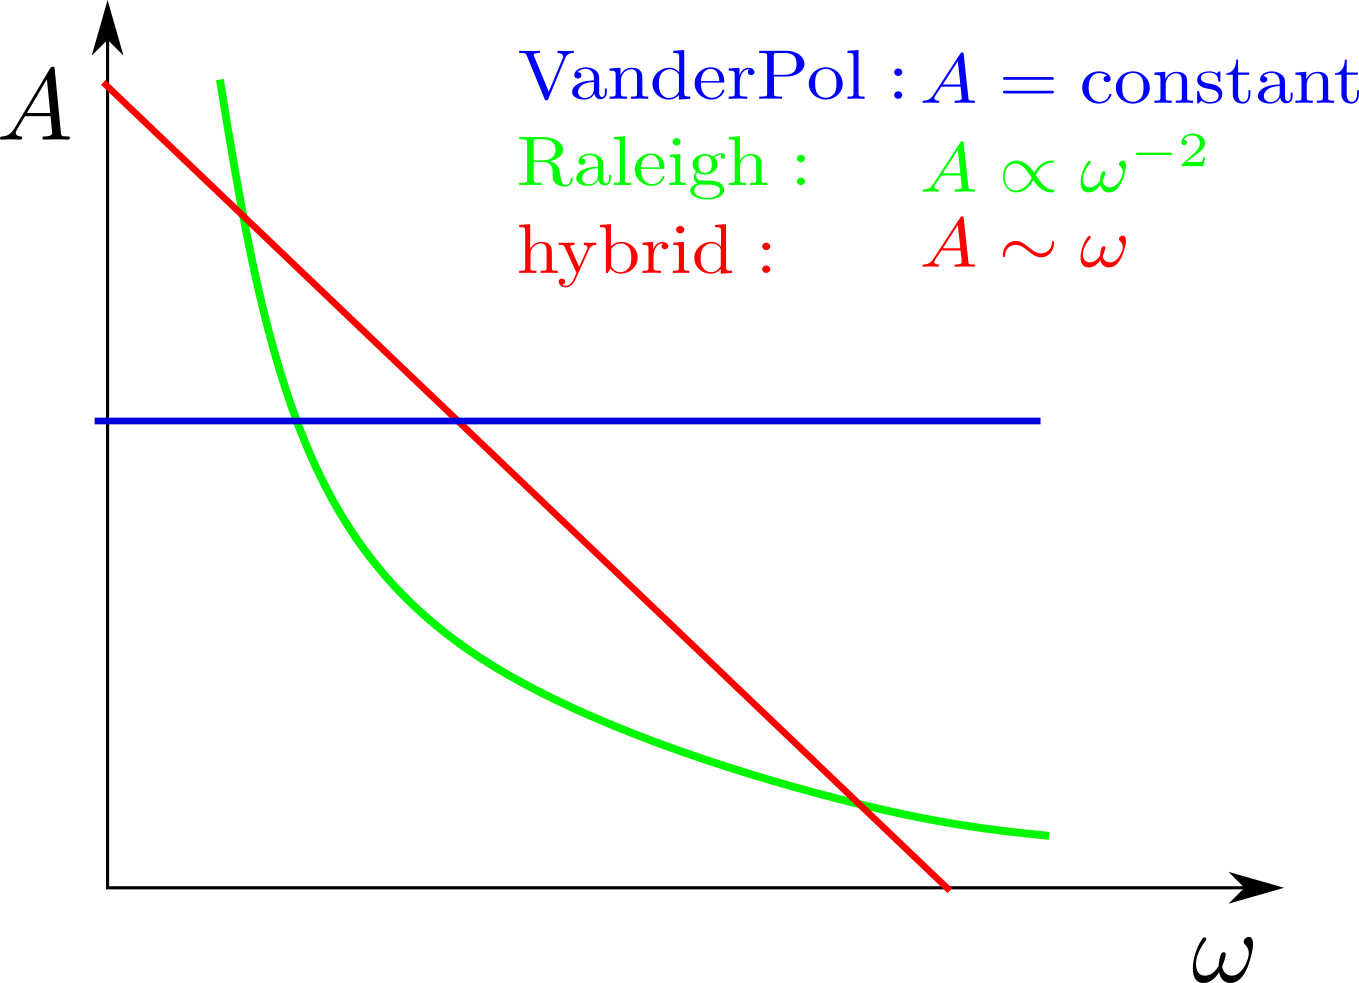
\includegraphics[width=2.3in]
{dynamical-sys/3-oscillator-spectra.png}
\caption{Spectra for 3 types of oscillators: Van der Pol, 
Raleigh and V-R hybrid.}
\label{fig-3-oscillator-spectra}
\end{figure}

\begin{claim}
Fig.\ref{fig-3-oscillator-spectra}  is correct.
\end{claim}
\proof

From Eq.(\ref{eq-spectrum-ho}), the
spectrum of a harmonic oscillator at its peak 
$\nu=\TIL{\omega}_0$ is approximately

\beq
S(\nu=\TIL{\omega}_0)\approx \frac{A^2}{4\gamma^2}
\eeq
Hence, 

\beq
|\TIL{x}(\nu)|=\sqrt{S(\nu=\TIL{\omega}_0)}
\approx \frac{A}{2\gamma}
\eeq

Averaging $\TIL{\gamma}$ over time
using the fact that $\av{\cos^2(\omega t)}
=\av{\sin^2(\omega t)}=\frac{1}{2}$, we get


\beqa
\av{2\TIL{\gamma}} &=&
\av{2\gamma + V x^2 + R \dot{x}^2}
\\
&=& 
2\gamma + \frac{A^2}{2}(V  - \omega_0^2 R)
\eeqa
so

\beq
|\TIL{x}(\nu=\omega_0)|\approx
\frac{A}{2[\gamma + \frac{A^2}{4}
(V-\omega_0^2 R)]}
\eeq

As $\omega_0\rarrow
\infty$
 
\begin{itemize}
\item if $V\neq 0$, $R=0$

\beq
|\TIL{x}|\propto \text{constant}
\eeq

\item if $V= 0$, $R< 0$

\beq
|\TIL{x}|\propto \frac{1}{\omega_0^2}
\eeq

\item if $V\neq 0$, $R< 0$ (V-R hybrid)

\beq
|\TIL{x}|\propto \frac{1}{V + \omega_0^2 R}
\eeq
\end{itemize}
\qed

We see from
this claim,
that $|\tilde{x}(\nu=\omega_0)|$
is flat for a linear or V oscillator,
but for a V-R hybrid oscillator, 
 it is shaped like a low pass filter with a region which is a reasonable approximation to a  line
 with negative slope.
 Ref.\cite{dynamical-fuchs} explains 
 that experimental findings for human limb motion
 are best modeled as V-R hybrid oscillations.
 



\section{Chaos}

A {\bf strange attractor}
is a set of attractor points that has fractal self-similarity 
properties.

\section{Famous Models}

\OtoAd

\subsection{Classical Mechanics}

Below, we illustrate Newton's, Lagrange's and
Hamilton's equations using a simple 1D harmonic
oscillator as an example. 
Its position 
will be denoted by $x$, its mass by $m$ and its momentum by
\beq
p=m\dot{x}
\eeq
The force applied to it is a spring force

\beq
F=-kx
\eeq
Its kinetic energy $T$
and potential energy $V$
are

\beq
T=\frac{m}{2}(\dot{x})^2\;, \;\;
V= \frac{k}{2}x^2
\eeq


\begin{itemize}
\item {\bf Newton's equation}

\beq
\xymatrix{
x\ar[dr]
&&
v\ar[dl]
\ar@/_2pc/[ddll]|\redplus
\\
&\frac{1}{m}F(x, v, t)\ar[dr]|\redplus
&
\\
\dot{x}
&&
\dot{v}
}
\left\{
\begin{array}{l}
\dot{x} = v
\\
\dot{v} = \frac{1}{m} F(x, v, t)
\end{array}
\right.
\eeq

For a harmonic oscillator, this becomes
\beq
\left\{
\begin{array}{l}
\dot{x} = v
\\
\dot{v} = -\frac{k}{m}x
\end{array}
\right.
\eeq


\item {\bf Euler-Lagrange equation}

\beq
\xymatrix{
\rvx\ar[dr]
\\
\dot{x}\ar[r]
&L\ar[r]\ar@/^1pc/[rr]
&\partial_x L\ar[dr]|\redplus
&\partial_{\dot{x}}L\ar[d]|{\;\redplus}
\\
&&&\frac{d}{dt}\left(\partial_{\dot{x}}L\right)
}
\left\{
\begin{array}{l}
\frac{d}{dt}\left(\partial_{\dot{x}}L\right)= \partial_x L
\end{array}
\right.
\eeq

For a harmonic oscillator, this becomes

\beq
L=T-V= 
\frac{m}{2}(\dot{x})^2 -  \frac{k}{2}x^2
\eeq

\beq
\partial_x L=-kx\;,\; \partial_{\dot{x}}L=m\dot{x}
\eeq

\beq
\left\{
m\ddot{x}=-kx
\right.
\eeq


\item {\bf Hamilton's equations}
\beq
\xymatrix{
x\ar[dr]
&&
p\ar[dl]
\\
\partial_p H\ar[d]|{\;\redplus}
&H\ar[l]\ar[r]
&\partial_x H\ar[d]|\redminus
\\
\dot{x}
&&
\dot{p}
}
\left\{
\begin{array}{l}
 \dot{x}=\partial_pH
\\
\dot{p} = -\partial_x H
\end{array}
\right.
\eeq

For a harmonic oscillator, this becomes

\beq
H= T+V = \frac{p^2}{2m} + \frac{k}{2}x^2
\eeq

\beq
\partial_x H = kx\;,\;\;
\partial_{p}H = \frac{p}{m}
\eeq

\beq
\left\{
\begin{array}{l}
\dot{x}=
\frac{p}{m}
\\
\dot{p}=-kx
\end{array}
\right.
\eeq
\end{itemize}


\subsection{FitzHugh-Nagumo model}
The  FitzHugh-Nagumo model is a reduced form of the Hodgkin-Huxley model for neuronal dynamics. It is given by

\beq
\xymatrix@R=3pc@C=3pc{
\rvx^3\ar[dr]|\redminus
&\rvx\ar[d]|{\;\redplus}
 \ar[dr]|\redplus
 \ar[l]
& \rvy\ar[d]|\redminus
\ar@/_1pc/[dl]|\redminus
\\
\ar[r]|\redplus
&\dot{\rvx}
&\dot{\rvy}
&\ar[l]|\redplus
}
\left\{
\begin{array}{l}
\dot{x} = x - \frac{x^3}{3} - y + R
\\
\dot{y} = \frac{1}{\tau} (x + a -b y)
\end{array}
\right.
\eeq
\OTO\cite{OTO}

\subsection{Heteroclinic Orbit Model}

\beq
\xymatrix{
\rvx \ar@/_2pc/[ddrr]|\redminus
&& \rvy\ar[dl]\ar[d]
\ar@/^2pc/[ddll]|\redplus
\ar[dl]
\\
&\rvy^3\ar@/_1pc/[dl]|\redminus
&\rvy^2\ar[d]|\redminus
\\
\dot{\rvx}
&&\dot{\rvy}
}
\left\{
\begin{array}{l}
\dot{x}= y - y^3
\\
\dot{y}=-x - y^2
\end{array}
\right.
\eeq
 \OTO\cite{OTO}



\subsection{Homoclinic Orbit Model}

\beq
\xymatrix{
\rvx\ar@/_2pc/[ddrr]|\redplus
\ar[dr]
&& \rvy\ar@/^2pc/[ddll]|\redplus
\\
&\rvx^3\ar@/^2pc/[dr]|\redminus
\\
\dot{\rvx}
&&\dot{\rvy}
}
\left\{
\begin{array}{l}
\dot{x}=y
\\
\dot{y} = x - x^3
\end{array}
\right.
\eeq
\OTO\cite{OTO}





\subsection{Lorenz system}

The  Lorenz system arises in fluid mechanics, laser physics, and other fields.
It is given by


\beq
\xymatrix@R=3pc@C=3pc{
\rvy\ar[d]|\redminus
\ar[r]
\ar@[green]@/^.8pc/[drr]|\redplus
&\bigotimes\ar[drrr]|\redplus
&\rvx\ar[l]
\ar[r]
\ar[d]|\redminus
\ar@[green]@/_.8pc/[dll]|\redplus
&\bigotimes\ar[dlll]|\redminus
&\rvz\ar[d]|\redminus
\ar[l]
\\
\dot{\rvy}
&&\dot{\rvx}
&&\dot{\rvz}
}
\left\{
\begin{array}{l}
\dot{x} = \sigma (y - x)
\\
\dot{y} = x(\rho - z) - y
\\ 
\dot{z} = xy - \beta z
\end{array}
\right.
\eeq
where $\sigma > 0$, $\rho > 0$, and $\beta > 0$ are parameters.
 \OTO\cite{OTO}




\subsection{Maxwell's equations}

\beq
\xymatrix{
\nabla\cdot\vec{E}\ar[d]|{\;\redplus}
&\vec{E} \ar[d]\ar[l]
& \vec{B}\ar[d]\ar[r]
&\nabla\cdot \vec{B}\ar[d]
\\
\frac{\rho}{\epsilon_0}
&\nabla\times\vec{E}\ar@/_1pc/[dr]|\redminus
&\nabla\times\vec{B}\ar@/_1pc/[dl]|\redplus
&0
\\
\frac{\vec{J}}{\epsilon_0}\ar[r]|\redminus
&\partial_t\vec{E}
&
\partial_t\vec{B}
}
\left\{
\begin{array}{l}
\frac{\rho}{\epsilon_0} = \nabla\cdot  \vec{E}
\\
0 = \nabla\cdot \vec{B}
\\
\partial_t\vec{B} = -\nabla\times \vec{E}
\\
\partial_t\vec{E}= \frac{1}{\mu_0\epsilon_0}
\left(\nabla\times \vec{B} -\mu_0 \vec{J}\right)
\end{array}
\right.
\eeq


\subsection{Navier-Stokes equation for incompressible fluid}

\beq
\xymatrix{
&\vec{u}\ar[d]
\ar[dr]
\ar[dl]
\\
\nabla \cdot \vec{u}\ar[d]
&\vec{u}\cdot\nabla \vec{u}\ar[d]|\redminus
&\nabla^2 \vec{u}\ar[dl]|\redplus
\\
0 &\partial_t\vec{u}&\ar[l]
}
\left\{
\begin{array}{l}
\partial_t \vec{u}=
-\vec{u}\cdot \nabla \vec{u}
+ \nu \nabla^2\vec{u}
-\frac{\nabla p}{\varrho}
+\frac{\vec{f}}{\varrho}
\\
\nabla\cdot \vec{u}=0
\end{array}
\right.
\eeq




\subsection{Predator Prey Model}
\label{sec-predator-prey}

The Predator-Prey model 
(a.k.a. Lotka-Volterra equations)
(See Ref\cite{wiki-volterra})
often arises in Biology and
Ecology.

\beq
\xymatrix{
\rvx \ar[d]|{\;\redplus}
\ar[r]
& 
\bigotimes
\ar[dl]|\redminus
\ar[dr]|{\redplus}
&\rvy \ar[d]|{\redminus}
\ar[l]
\\
\dot{\rvx}
&
&\dot{\rvy}
}
\left\{
\begin{array}{l}
\dot{x} = \alp x -\beta xy
\\
\dot{y} = -\gamma y + \delta xy
\end{array}
\right.
\eeq
\OTO\cite{OTO}

\subsection{Schr\"{o}dinger's  equation}

Schr\"{o}dinger's equation for
the wavefunction $\Psi(x,t)$ of a point particle
of mass $m$ in a potential $V(x, t)$ in 1D is
\beq
\xymatrix@R=1pc{
&\Psi\ar[dd]
\ar[dl]
\\
\partial_x^2\Psi
\ar[dr]|\redminus
\\
&i\hbar \partial_t \Psi
}
\quad
\left\{
i\hbar\partial_t \Psi =\left[
- \frac{1}{2m}\partial_x^2 + V
\right]\Psi
\right.
\eeq

\subsection{Van der Pol oscillator}


\beq
\xymatrix@C=3pc{
\rvx\ar@/_1pc/[drrr]|\redminus 
\ar[r]
&(1-\rvx^2)\ar[r]
&\bigotimes\ar[dll]|\redplus
&\rvv\ar[dlll]|\redplus
\ar[l]
\\
\dot{\rvx}
&&&\dot{\rvv}
&\ar[l]
}
\left\{
\begin{array}{l}
\dot{x}=v
\\
\dot{v}= \mu (1-x^2)v - x + A \sin(\omega t)
\end{array}
\right.
\eeq \OTO\cite{OTO}

